%%%%%%%%%%%%%%%%%%%%%%%%%%%%%%%%%%%%%%%%%%%%%%%%%%%%%%%%%%%%%%%%%%%%%%%%
%    INSTITUTE OF PHYSICS PUBLISHING                                   %
%                                                                      %
%   `Preparing an article for publication in an Institute of Physics   %
%    Publishing journal using LaTeX'                                   %
%                                                                      %
%    LaTeX source code `ioplau2e.tex' used to generate `author         %
%    guidelines', the documentation explaining and demonstrating use   %
%    of the Institute of Physics Publishing LaTeX preprint files       %
%    `iopart.cls, iopart12.clo and iopart10.clo'.                      %
%                                                                      %
%    `ioplau2e.tex' itself uses LaTeX with `iopart.cls'                %
%                                                                      %
%%%%%%%%%%%%%%%%%%%%%%%%%%%%%%%%%%
%
%
% First we have a character check
%
% ! exclamation mark    " double quote  
% # hash                ` opening quote (grave)
% & ampersand           ' closing quote (acute)
% $ dollar              % percent       
% ( open parenthesis    ) close paren.  
% - hyphen              = equals sign
% | vertical bar        ~ tilde         
% @ at sign             _ underscore
% { open curly brace    } close curly   
% [ open square         ] close square bracket
% + plus sign           ; semi-colon    
% * asterisk            : colon
% < open angle bracket  > close angle   
% , comma               . full stop
% ? question mark       / forward slash 
% \ backslash           ^ circumflex
%
% ABCDEFGHIJKLMNOPQRSTUVWXYZ 
% abcdefghijklmnopqrstuvwxyz 
% 1234567890
%
%%%%%%%%%%%%%%%%%%%%%%%%%%%%%%%%%%%%%%%%%%%%%%%%%%%%%%%%%%%%%%%%%%%
%
\documentclass[12pt]{iopart}
\newcommand{\gguide}{{\it Preparing graphics for IOP Publishing journals}}
%Uncomment next line if AMS fonts required
%\usepackage{iopams}  
\usepackage{graphicx}% Include figure files
% \usepackage{amsmath,amssymb}
\usepackage{subcaption}
\usepackage[dvipsnames]{xcolor}
% \linespread{1.5}
\begin{document}

\title[Plasma Sources Science and Technology]{Development of a Stark Shift Measurement Technique using Excited-State Oxygen Atoms to Determine Electron Number Density in Shock Heated O$_2$/Ar above 10,000 K }

\author{Yang Li }
\address{High Temperature Gasdynamics Laboratory, Stanford University}
% \ead{yli28@stanford.edu}
\author{Shengkai Wang }
\address{State Key Laboratory for Turbulence and Complex Systems, College of Engineering, Peking University, Beijing, 100871, China}
\address{Beijing Innovation Center for Engineering Science and Advanced Technology, Peking University, Beijing, 100871, China}
\author{Christopher L. Strand }
\address{High Temperature Gasdynamics Laboratory, Stanford University}
\author{Ronald K. Hanson }
\address{High Temperature Gasdynamics Laboratory, Stanford University}


% \ead{submissions@iop.org}
\vspace{10pt}
\begin{indented}
\item[]November 2020
\end{indented}

\begin{abstract} 
We present measurements of electron number density, $n_e$, in partially ionized gases containing electronically excited atomic oxygen, at nominal translational temperatures between 10,100 - 11,200 K. The measurements were based on the Stark shift of the O($^5$P$_{3}$) to O($^5$D$_{2,3,4}^0$) transition at 926 nm. The current work scanned the laser across the transition and utilized the Stark shift of the absorbance for robust determination of $n_e$. The measurements were conducted in a shock-heated 1\% O$_2$/Ar mixture, with a measurement time resolution of 20 $\mu s$. A line-center shift of -0.06 cm$^{-1}$ was observed at around 500 $\mu s$ of the test time after the mixture was instantaneously heated to 11,200 K by the reflected shock wave, which corresponds to an electron number density increase from 0 to 2$\times 10^{21}$ m$^{-3}$ due to collisional ionization. The measurement method and resulting data may be of interest in future studies of high-temperature air flows.
\end{abstract}

\section{Introduction}
The current work focuses on the excitation kinetics of argon-diluted atomic oxygen at high temperatures (T $>$ 10,000 K), which can be studied behind reflected shock waves. The excitation process is usually initiated with collisions of charge-neutral heavy particles such as argon, followed by the generation of free electrons from collisional ionization of argon and atomic oxygen, which subsequently accelerate the excitation process as the electrons have much higher collision efficiency. The heavy-particle excitation processes have been studied previously at Stanford University\cite{Nations2016} over 5400 - 7500 K where the free electrons are sparse. The electron-impact excitation processes were explored further in a more recent study\cite{Li2019_modeling} at much higher temperatures (8000 - 10000 K), where the formation of free electrons was no longer negligible, as manifested in the interesting yet complex multi-stage dynamics of population evolution in the electronically excited oxygen states. The temporal evolution of the number density of free electrons, $n_e$, holds the key to unravelling the kinetics of this system, the measurement of which is the main goal of this study. 

Many techniques have been developed for an electron number density diagnostic, such as Langmuir probes\cite{Griem1964}, microwave techniques\cite{jahn_1962_microwave,Schneider2005}, interferometry\cite{becker2005_nonequilibrium_air}, Thompson scattering\cite{engeln_2020}, Optical Emission Spectroscopy (OES)\cite{Laux2003,Konjevic2012} and laser absorption spectroscopy(LAS)\cite{Baer1992c,baer1992d, Baer1993_semiconductor}. They all have their own strengths and weaknesses and are most useful within a limited range of electron number density, species, time and spatial resolution. To study the collisional excitation kinetics of atomic oxygen, an electron number density diagnostic tool is developed in the present work using the Stark shift of excited-state atomic oxygen absorption transitions. The electron number density measured in the current study is in the range of $1\times10^{20}<n_e<3\times10^{21}$m$^{-3}$, limited by the translational temperature behind the reflected shock waves on the higher end. 

Balmer series OES of hydrogen atoms\cite{Laux2003,Lemal2016,grinstead2008,cruden2009, cruden2012} has been widely used for $n_e$ diagnostics in high-enthalpy air experiments because of the reliable Stark broadening parameters for atomic hydrogen. For applications without naturally occurring hydrogen, H$_2$ or water need to be seeded into the system, which may potentially alter the kinetics of the  species that one is interested in originally. For example, Cruden\cite{cruden2009} measured the snap-shot spatial profile of the electron number density (on the order of 10$^{22}$m$^{-3}$) behind a 10 km/s incident shock in the Electric Arc Shock Tube at NASA Ames by seeding 0.1\% H$_2$ and fitting the Stark broadening of H$_{\alpha}$ emission profile with a Lorentzian fit. Later, Cruden\cite{cruden2012} used the Stark broadening of five different emission lines of H, N, O atoms to determine the electron number density from 10$^{20}$ - 10$^{22}$ m$^{-3}$ over a wider pressure and shock velocity range.  

LAS, as explored further in this work, may also be used to determine $n_e$ through the Stark broadening and shift of absorption transitions\cite{Baer1992c,baer1992d,Baer1993_semiconductor,Konjevic1999}. Baer et al. determined the electron number density using the Stark width and shift of the argon 4s $^3 $P$_2\rightarrow$ 4p $^3$D$_3$ and 4s $^3 $P$_1\rightarrow$ 4p $^3$D$_1$ transitions  at 811.5 nm and 810.4 nm in an atmospheric pressure plasma torch\cite{Baer1992c}. The electron number density inferred from four different components were mutually consistent within the 15\% experimental uncertainty. Later, the same group utilized laser-induced fluorescence of the transition at 810.4 nm  to measure the spatially-resolved electron number density\cite{baer1992d}. The absorption lineshapes of the atomic oxygen and argon 3s $^5 $S$_2^0\rightarrow$ 3p $^5$P$_3$ and 4s $^3 $P$_1\rightarrow$ 4p $^3$D$_2$ transition were used to determine electron number density in a 12\% O$_2$/argon inductively coupled atmospheric-pressure plasma\cite{Baer1993_semiconductor}. Notably, the Stark shift of the atomic oxygen transition was also observed by these authors but not utilized for $n_e$ determination, because of the small magnitudes of Stark shift and the unknown contribution of van der Waals shift to the total shift.

It is known that spectral linewidth fitting can be prone to measurement noise, especially when the lineshape is simultaneously broadened by multiple mechanisms. In high-temperature, partially-ionized environments where Doppler broadening, van der Waals broadening and Stark broadening co-exist, it is often difficult to accurately separate the three effects, as reported in earlier OES\cite{xingxingwang2018,Liebeskind1993b} and LAS\cite{Griem1964} studies. To mitigate this problem, in the current study we introduced a different measurement strategy for $n_e$, that is to utilize the line-center shift found following lineshape fitting. Compared to the linewidth, the line-center shift is insensitive to the relative magnitudes of different broadening mechanisms and could be measured with high accuracy. More specifically, we determined the time-history of $n_e$ by fitting the Stark shift from the measured absorption lineshape of the O(3p $^5$P$_{3}$) to O(3d $^5$D$_{2,3,4}^0$) transition at 926 nm. The current study has achieved a time-resolution of 20 $\mu$s, which can be further improved by increasing the scanning rate of the laser. The experimental details and representative results of the current study are discussed in the next sections.

\section{Experimental Setup and Methods}
\subsection{Experimental set up}
\begin{figure}[h]
  \centering
     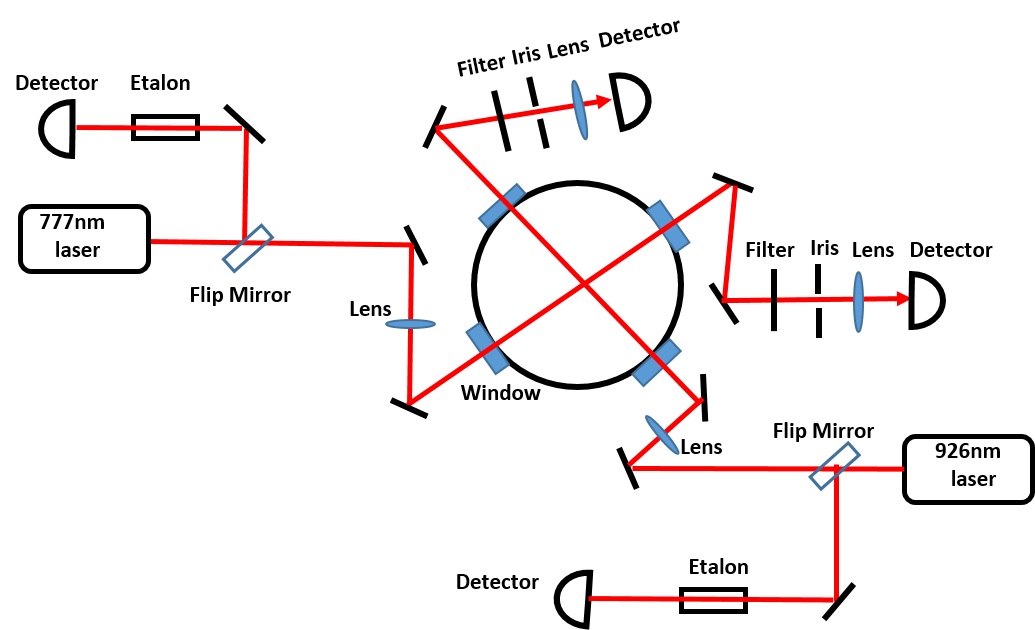
\includegraphics[width=0.6\textwidth]{schematic.png}
    \caption{\label{fig:schematic}  The schematic of the experimental setup. 
    }
\end{figure}
A schematic of the experimental setup is shown in figure \ref{fig:schematic}. The shock tube used to generate controlled temperatures of 10,100-11,200K has been discussed in previous papers\cite{Li2019_modeling,nations2015_new}. The driven section was filled with 1\% O$_2$/Ar (Praxair) to 0.7-1 torr. The driver section was filled with He (Praxair) to approximate 130-160 psia until the diaphragm ruptured. The incident shock traveled down the driven section and its velocity was measured by five piezoelectric pressure transducers. The incident shock then hit the endwall and was reflected. The temperature and pressure immediately behind the reflected shock was calculated using an in-house code, Frozen-chemistry shock calculator (FROSH). The pressure trace was recorded with a Kistler pressure sensor. The typical thermodynamic condition is 10,100-11,200 K and 0.3-0.5 atm. The typical test time is 400 - 500 $\mu$s, limited by the time when the reflected shock from the contact surface arrives.

Two distributed-feedback (DFB) lasers were used to probe the excited-state oxygen atoms: one at 777 nm targeting at the O(3s $^5$S$^0$) to O(3p $^5$P$_{3}$) transition  and the other at 926 nm targeting at the O(3p $^5$P$_{3}$) to O(3d $^5$D$_{2,3,4}^0$) transition; see figure \ref{fig:energy_level}. The lasers were modulated using a 25 kHz triangle wave to achieve a measurement time resolution of 20 $\mu$s by performing a measurement on both the up and down scans of the lasers. The 926 and 777 nm lasers were propagated through two pairs of UV fused silica and wedged CaF$_2$ windows located 5 mm away from the shock tube end wall. The transmitted light was recorded by two photodiode detectors (Thorlabs PDA36A, $f_{-3dB} \ge 1.6$MHz). The data acquisition system recorded the detector signal at a sampling rate of 100 MHz.

\begin{figure}[h]
  \centering
     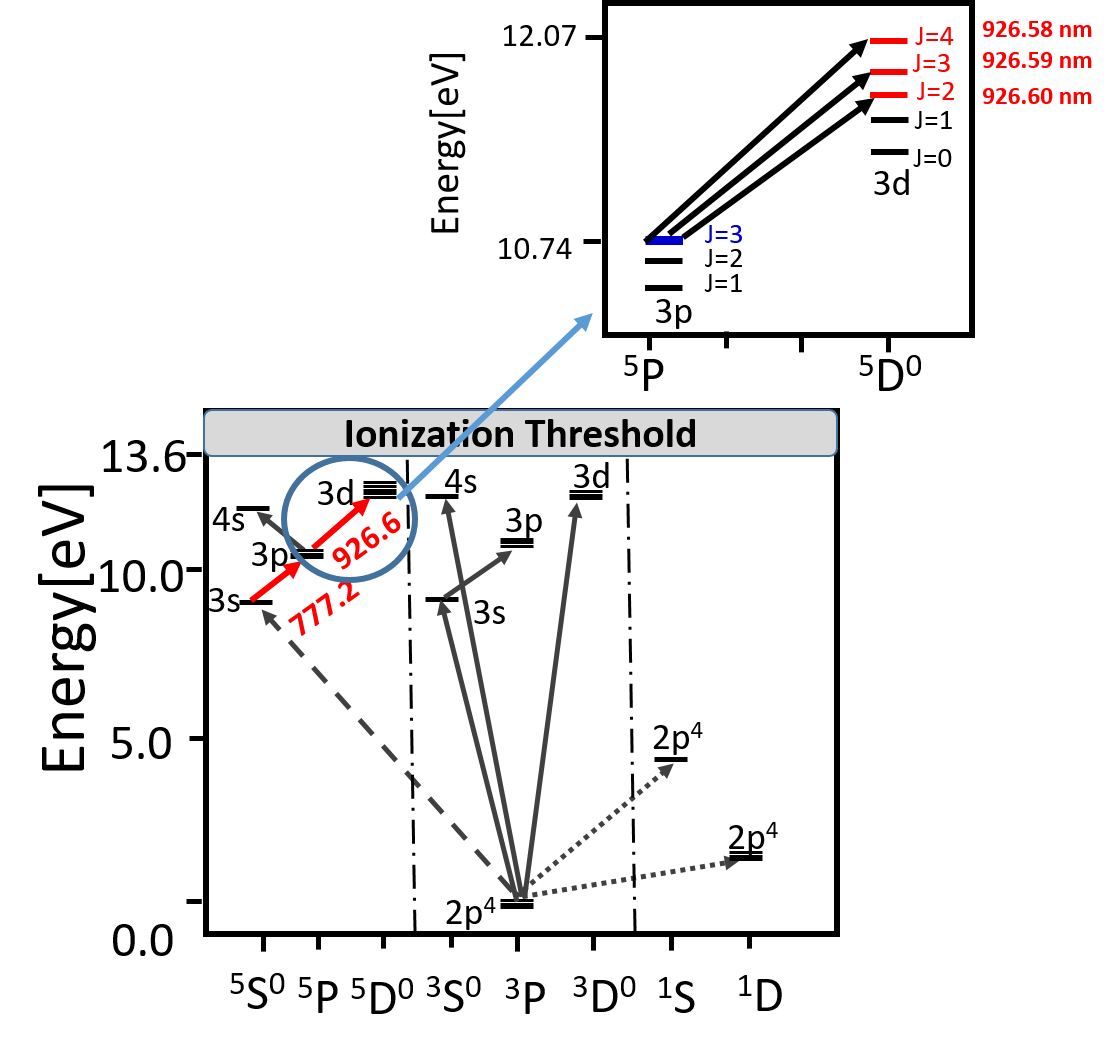
\includegraphics[width=0.6\textwidth]{energy_level_new.png}
    \caption{\label{fig:energy_level}  Energy level of the atomic oxygen. The targeted O(3p $^5$P$_{3}$) to O(3d $^5$D$_{2,3,4}^0$) transition at 926 nm and the  O(3s $^5$S$^0$) to O(3p $^5$P$_{3}$) transition at 777 nm are shown in red. The 926 nm transition lineshape includes three blended lines: lower energy level J=3 to upper energy level J=2,3,4. 
    The energy level O(3s $^5$S$^0$), O(3p $^5$P$_{3}$) and O(3d $^5$D$_{2,3,4}^0$) are the 4$^{th}$, 6$^{th}$ and 10$^{th}$ energy level for the atomic oxygen, respectively. 
    }
\end{figure}

\subsection{O* absorption spectroscopy }
The spectral absorbance $\alpha_{\nu}$ is determined from the transmitted laser intensity as shown in the following expression.

\begin{equation}\label{eq:beer's_law}
    \alpha_{\nu} = - \ln (\frac{I_t}{I_0}) = n_l L\sum_j S_j \phi_j(\nu)
\end{equation}
where $I_t$ and $I_0$ are the transmitted light intensity with and without the absorbing species, respectively;  $\alpha_{\nu}$ is the absorbance; $n_l$ is the number density of atomic oxygen in the specific quantum states, i.e. O(3s $^5$S$^0$) or O(3p $^5$P$_{3}$), probed by laser absorption at 777 nm or 926 nm, respectively; $L$ = 15.24 cm is the optical path length; $\phi_j(\nu)$ is the lineshape of the absorbance for transition $j$; $S_j$ is the linestrength of the transition $j$, which is calculated below.
\begin{equation}
S_j [\textrm{cm/molec}] = \frac{c}{8\pi\nu_{0,j}^2}  A_{j} \frac{g_{u,j}}{g_{l,j}}[1-\exp(-\frac{h\nu_{0,j}}{k_BT})]  
\end{equation}
where $c$ is speed of light in cm/s, $\nu_{0,j}$ is the vacuum transition frequency in Hz, $A_{j},g_{u,j},g_{l,j}$ are Einstein coefficient and upper and lower state degeneracy summarized in Table \ref{tab:Spectroscopic paprameters}. For the 926 nm transition, the summation runs over $j=1,2,3$, corresponding to the upper level J = 2, 3 ,4. $j=1$ for the 777 nm transition.

% For tables use
\begin{table*}
\centering
\caption{Spectroscopic parameters for atomic oxygen transitions\cite{nist_o_lines}. $A_{ul}$ is the Einstein coefficient of the transition between states \textit{u} and \textit{l}.  $E_l$ and  $E_u$ are the energy of the states \textit{l} and \textit{u}.  $g_l$ and $g_u$ are the degeneracy of the \textit{l} and \textit{u} states.  }
\label{tab:Spectroscopic paprameters}       % Give a unique label
% For LaTeX tables use
\begin{tabular}{ccccccc}
\hline\noalign{\smallskip}
Transition & Ritz Wavelength in Air(nm) & $A_{ul}( \textrm{s}^{-1}$)  & $E_l$(cm$^{-1}$)   & $E_u$(cm$^{-1}$)  & $g_l$ & $g_u$\\
\noalign{\smallskip}\hline\noalign{\smallskip}
3s $^5$S - 3p $^5$P$_{3}$ &777.194 & 3.69 $\times10^7$  &73768.200   &86631.454  &5  &7  \\
3p $^5$P$_{3}$ - 3d $^5$D$_{2}^0$  & 926.60 &2.97 $\times10^6$ & 86631.454   &97420.839  &7  &5\\
3p $^5$P$_{3}$ - 3d $^5$D$_{3}^0$ &926.59 & 1.48 $\times10^7$ & 86631.454    &97420.716   &7  &7\\
3p $^5$P$_{3}$ - 3d $^5$D$_{4}^0$ &926.58   & 4.45$\times10^7$  & 86631.454   &97420.630 	  &7  &9  \\
\noalign{\smallskip}\hline
\end{tabular}
% Or use
% \vspace*{5cm}  % with the correct table height
\end{table*}

The lineshape of the absorption spectrum is the result of various broadening mechanisms, including natural broadening, Doppler broadening, resonance broadening, van der Waals broadening and Stark broadening\cite{Laux2003}.
Natural broadening is on the order of 0.0002 cm$^{-1}$, which is three orders of magnitude smaller than the Doppler broadening and therefore neglected in the current work.

Resonance broadening originates from the collisions with identical particles where the perturber is connected to its ground state with an allowed transition\cite{Griem1964}. This broadening is weak for the current two transitions because there are no allowed transitions coupling the O(3s $^5$S$^0$) and O(3p $^5$P$_{3}$) states to the ground state. Resonance broadening is also neglected in the current work.

The Doppler broadening full width half maximum (FWHM), $\Delta \nu_{D}$ is given by\cite{Hanson2016}
\begin{equation}
    \label{eq:doppler_width}
    \Delta \nu_{D} = \nu_0 (\frac{8kT\ln 2}{mc^2})^{\frac{1}{2}}
     = 7.16\times10^{-7} \nu_0 (\frac{T}{M_O})^{\frac{1}{2}}
\end{equation}
where $\nu_0$ is the transition line-center frequency in cm$^{-1}$, T is the translational temperature in K, $M_O$ is the molecular weight of atomic oxygen. 

The FWHM linewidth of the van der Waals broadening (collisional broadening by charge-neutral particles), $\Delta \nu_{vdw}$ for an absorber surrounded by perturbers \textit{p} is given by\cite{Griem1964}
 \begin{equation}\label{eq:vdw_broadening}
     \Delta \nu_{vdw} \approx 0.98 \frac{1}{c}(\frac{9\pi \hbar^5 \overline{R^2_{\alpha}}}{16 m_e^3 })^{\frac{2}{5}} (\frac{8k_BT}{\pi})^{\frac{3}{10}}\frac{P}{k_B T}\sum_p \frac{X_p}{E_p^{\frac{4}{5}} (m^*_{ap})^{\frac{3}{10}}} 
 \end{equation}
where $m^*_{ap}$ is the reduced mass for the collisional partner and the absorber, $E_p$ is the the energy gap between the first excited state of the perturber connected with its ground state by an allowed transition, $P$ is the total pressure, $X_P$ is the mole fraction of the perturbers. The matrix element $\overline{R^2_{\alpha}}$ is given by 

\begin{equation}
    \overline{R^2_{\alpha}} = \frac{1}{2} \frac{E_H}{E_{\infty} - E_{\alpha} } [5\frac{z^2E_H}{E_{\infty} - E_{\alpha}} + 1 - 3l_{\alpha}(l_{\alpha}+ 1)] 
\end{equation}
where z is the number of effective charges. $E_{\infty}=E_H = 13.6$eV, $ E_{\alpha}$ is the excitation potential of the upper state of the transition.

Similarly, collisions by charged particles will cause Stark broadening, the influence of which will be further discussed in the next section. Both the van der Waals broadening and the Stark broadening result in a Lorentzian lineshape, which is often characterized by the collisional broadening coefficient $2\gamma$. In the current study, the total collisional broadening is simply the summation of the van der Waals broadening $\Delta \nu_{vdw}$, and the Stark broadening $\Delta \nu_{s}$.

\begin{equation}\label{eq:2gamma}
        \Delta \nu_c = \Delta \nu_{vdw} + \Delta \nu_s    = 2\gamma_{eff} P
\end{equation}
where $P$ is the total pressure of the system, $2\gamma_{eff}$ is the effective collisional broadening coefficient accounting for the Stark broadening.

\begin{figure}[h]
  \centering
     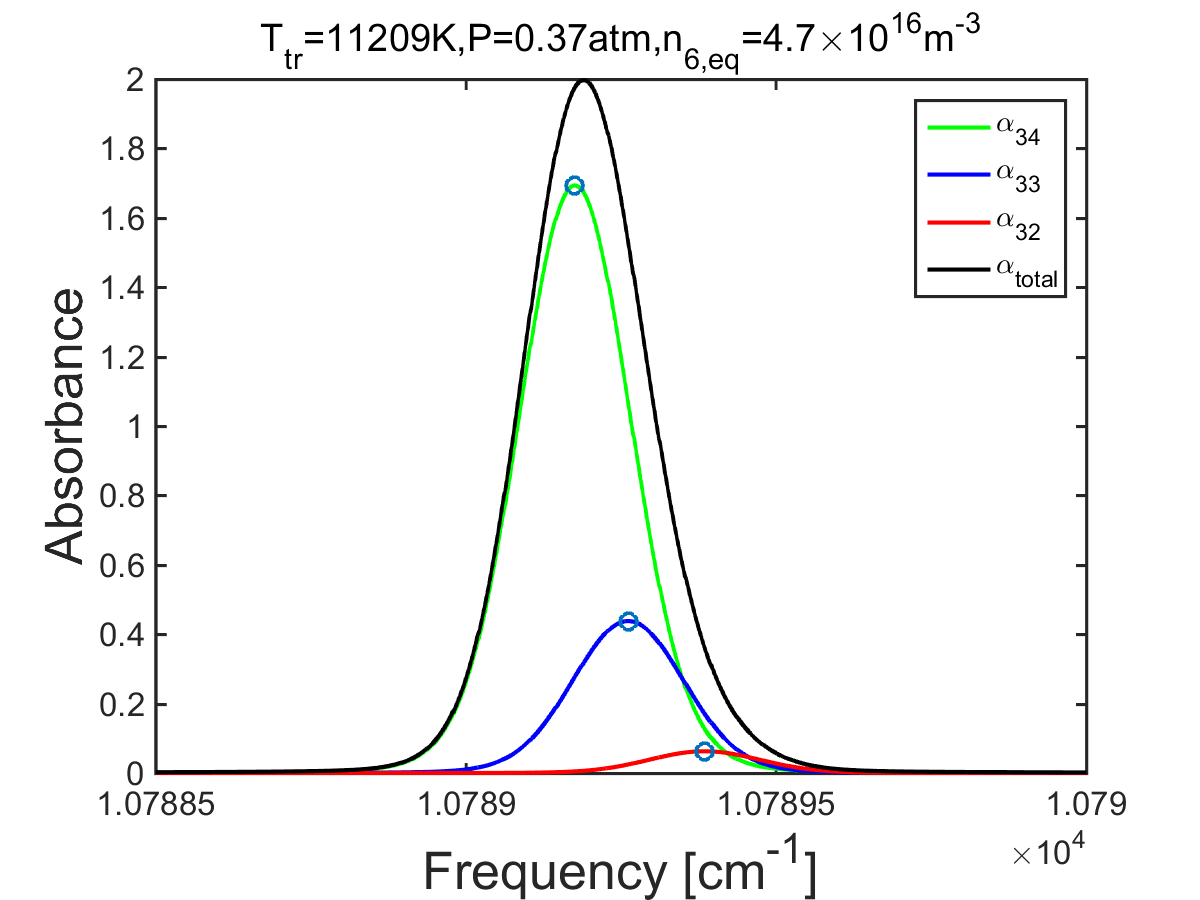
\includegraphics[width=0.6\textwidth]{abs_sim.png}    \caption{\label{fig:lineshape_eq} The absorbance calculated using an estimated Voigt lineshape and equilibrium population of the O(3p $^5$P$_{3}$) state assuming Boltzmann distribution at the initial translational temperature of 11209 K and initial pressure of 0.37 atm. Optical path length is 15.24 cm for the current shock tube. The line-centers of the three blended transitions are marked by circles. }
\end{figure}
Figure \ref{fig:energy_level} shows that the absorbance of 926 nm transition is blended by the three upper energy levels: O(3d $^5$D$_{2}^0$), O(3d $^5$D$_{3}^0$), and O(3d $^5$D$_{4}^0$).  Figure \ref{fig:lineshape_eq} shows the calculated absorbance of the 926 nm transition at 11209 K, 0.37 atm assuming a Boltzmann distribution of excited-state populations, considering only Doppler broadening and van der Waals broadening estimated from the measured 777 nm transition $2\gamma$\cite{nations2015_new}. Stark shift and broadening is not included in this figure. The line-center positions for the three transitions are taken from NIST database. $\alpha_{32},\alpha_{33},\alpha_{34}$ correspond to the absorbances of the three transitions. The total absorbance is simply the linear superposition of the three.


\subsection{Stark broadening/shift}
Griem\cite{Griem1964} and Huddleston\cite{huddlestone_plasma_1965} studied the theory of the Stark effect in great detail. Their main results are reproduced below.

The FWHM of atomic lines(in $\AA$) is given by\cite{huddlestone_plasma_1965, baer1992d, griem_2012_parameters}.
\begin{equation}\label{eq:stark_broadening}
    \Delta\lambda_{Stark} \approx  2 [1 + 1.75 \times 10^{-4} n_e ^{\frac{1}{4}} \alpha (1-0.068 n_e ^{\frac{1}{6}}T_e^{-\frac{1}{2}})]10^{-16}wn_e
\end{equation}
and the shift(in $\AA$)
\begin{equation}\label{eq:stark_shift}
    \delta\lambda_{Stark} \approx [(\frac{d}{w}) \pm 2.0 \times 10^{-4} n_e^{\frac{1}{4}} \alpha (1-0.068 n_e ^{\frac{1}{6}}T_e^{-\frac{1}{2}})]10^{-16}wn_e
\end{equation}
where $n_e$ is the electron number density, $T_e$ is the electron temperature, $w$ is the electron impact half-width, $\frac{d}{w}$ is the relative electron-impact shift, and $\alpha$ is the ion-broadening parameter.  The plus sign in equation \ref{eq:stark_shift} is used for the current transition. The minus sign in equation \ref{eq:stark_shift} applies only to the high temperature range of those few lines which have a negative $\frac{d}{w}$ term at low temperatures. The shifts are generally positive, i.e., toward increasing wavelength (red shifts). To convert the units from $\AA$ to cm$^{-1}$, $\delta_\nu = - \frac{\delta\lambda_{Stark}}{\lambda^2}$.

The values of $w,d$ for the 777 and 926 nm transitions at 10,000K are reproduced in Table \ref{tab:Stark_parameters} following Griem's book\cite{griem_2012_parameters}. Note these values may not be as accurate as hydrogen Stark parameters because of the complex structure of atomic oxygen. Few experimental data for these parameters were found in the literature. Electron number density inferred from the Stark shift and broadening of the 777 and 926 nm transitions were mutually consistent as shown  in the ``Results" section, which validated these formulas to some extent. 

\begin{table}[h]
\centering
\caption{\label{tab:Stark_parameters} The value of the Stark parameters  in equation \ref{eq:stark_broadening} and \ref{eq:stark_shift}\cite{griem_2012_parameters} at 10,000K.}
% \begin{ruledtabular}
\begin{tabular}{ccc}
Parameter & 777 nm     &926 nm\\\hline
 w($\AA$) & 0.0315    &0.222   \\
 d($\AA$) & 0.0143    &0.228     \\
 $\alpha$ & 0.012     &0.05\\
\end{tabular}
% \end{ruledtabular}
\end{table}

Table \ref{tab:Stark_parameters} shows that the broadening width and shift of the 777 nm transition are approximately 10 times smaller than those of the 926 nm transition. This difference is observed in our measured Stark shift shown in the ``Results" section. The 926 nm transition has a width-to-shift ratio on the order of 1, which makes its Stark shift very sensitive to the electron number density. 

As a rule of thumb, the approximate expressions \ref{eq:stark_broadening} and \ref{eq:stark_shift} are sufficiently accurate, as long as the following three conditions are fulfilled\cite{Baer1992c}:

\begin{equation}\label{eq:criterion1}
    10^{-4}\times\alpha n_e^{\frac{1}{4}} < 0.5
\end{equation}
\begin{equation}\label{eq:criterion2}
    \sigma >1
\end{equation}
\begin{equation}\label{eq:criterion3}
    R<0.8
\end{equation}
where the parameter $R$ is given by 
\begin{equation}
    R = 9.0 \times 10^{-2} n_e^{\frac{1}{6}}T^{-\frac{1}{2}}
\end{equation}
and the parameter $\sigma$ is given by
\begin{equation}
    \sigma = \frac{3\pi}{v_ev_i}\left(\frac{hn^2}{2\pi m_ez}\right)^2 \frac{n_e}{n_i^{1/3}}
\end{equation}
where $v_e,v_i$ are the electron and ion mean velocities; z is the effective nuclear charge; n is the effective principal quantum number of the upper state of the transition; $n_e,n_i$ are the number densities of the electron and ions.


Applying these criteria to conditions relevant to the experiments performed here (T=10,000 K), the minimum electron number density for which the criteria hold is $1.6\times10^{21}$m$^{-3}$. The range of $n_e$ inferred from the experiments performed here using these expressions is $1\times10^{20}$ to $2.5\times10^{21}$ m$^{-3}$. In the lowest density cases, equation \ref{eq:criterion2} is violated ($\sigma=0.15$). Thus the uncertainty in equation \ref{eq:stark_shift} is higher when used to infer low electron number density values.


Ideally, the electron temperature $T_e$ should be used in equations \ref{eq:stark_broadening} and \ref{eq:stark_shift}. The initial translational temperature is used here instead for simplicity.  The Stark shift error caused by the discrepancy between $T_e$ and $T_{tr}$ is small because the Stark shift and broadening are only weakly dependent on temperature.  Figure \ref{fig:delta_vs_Tdependance} shows that the change in Stark shift is smaller than 13\% when electron temperature changes from 5,000 to 10,000K. 
\begin{figure}[h]
  \centering
    \begin{subfigure}[b]{0.4\textwidth}
     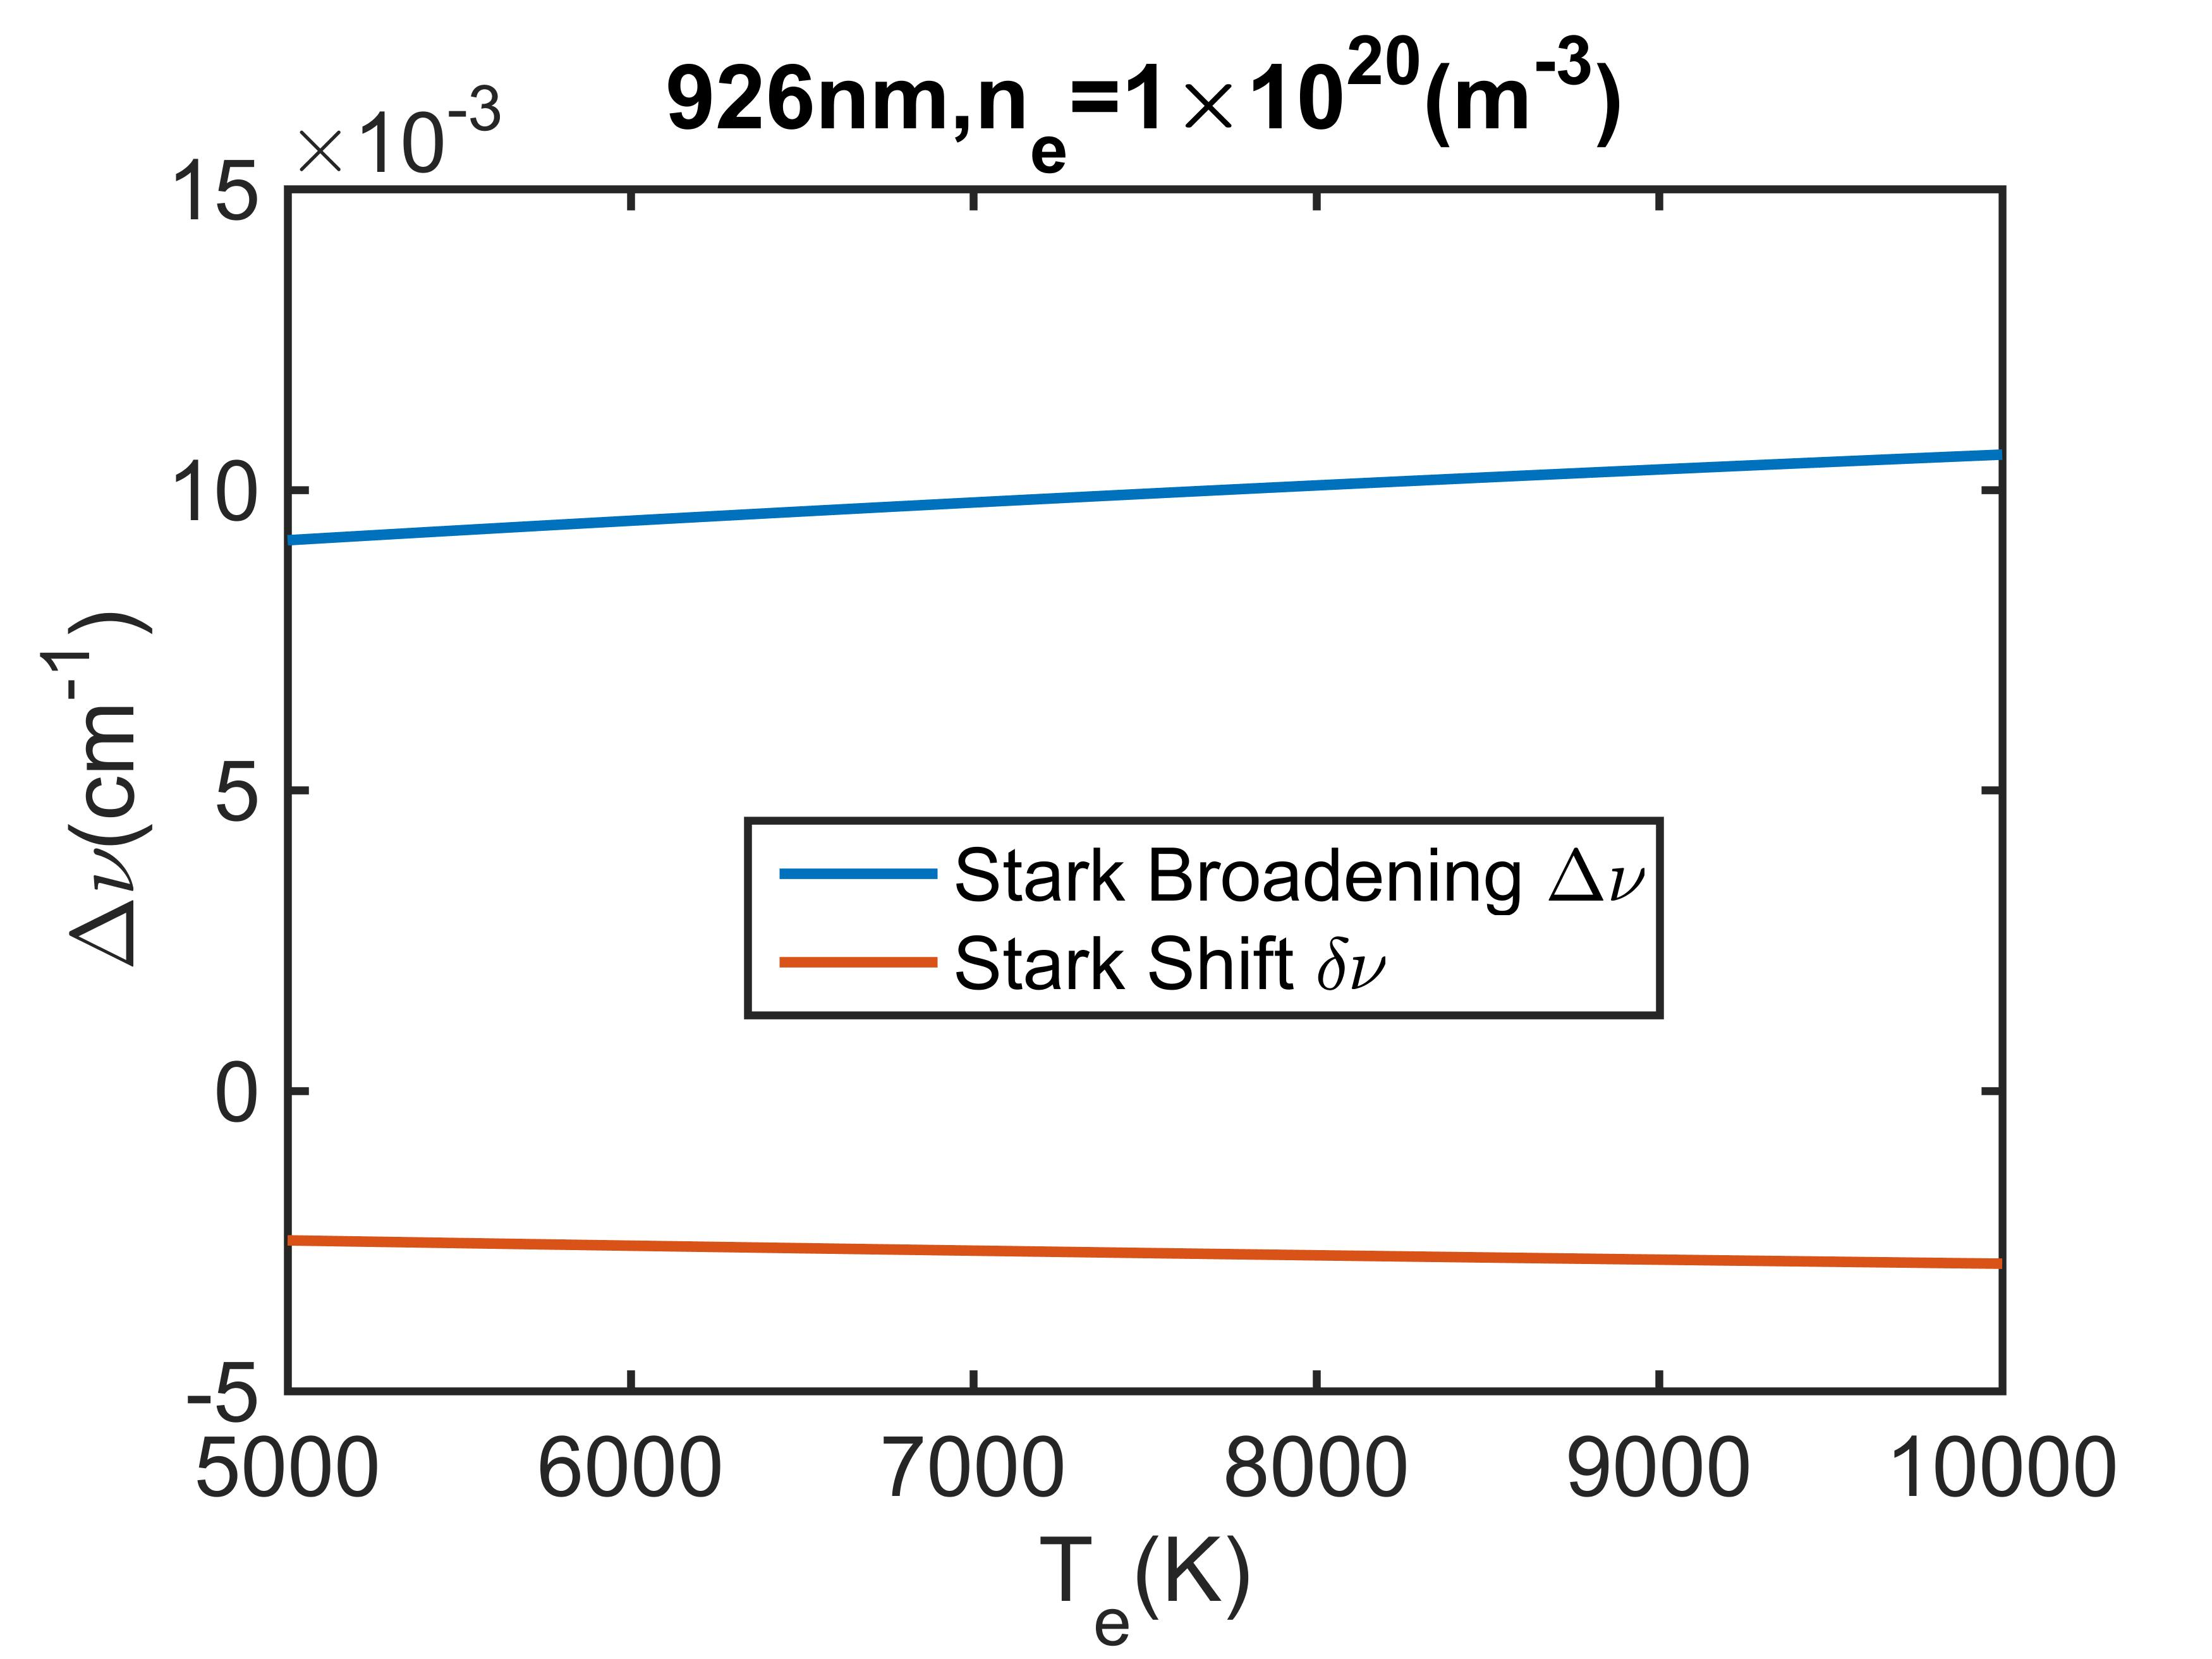
\includegraphics[width=\textwidth]{delta_vs_Tdependance_926.jpg}
    \caption{\label{fig:delta_vs_Tdependance_926} }  
      \end{subfigure} %
      \begin{subfigure}[b]{0.4\textwidth}
     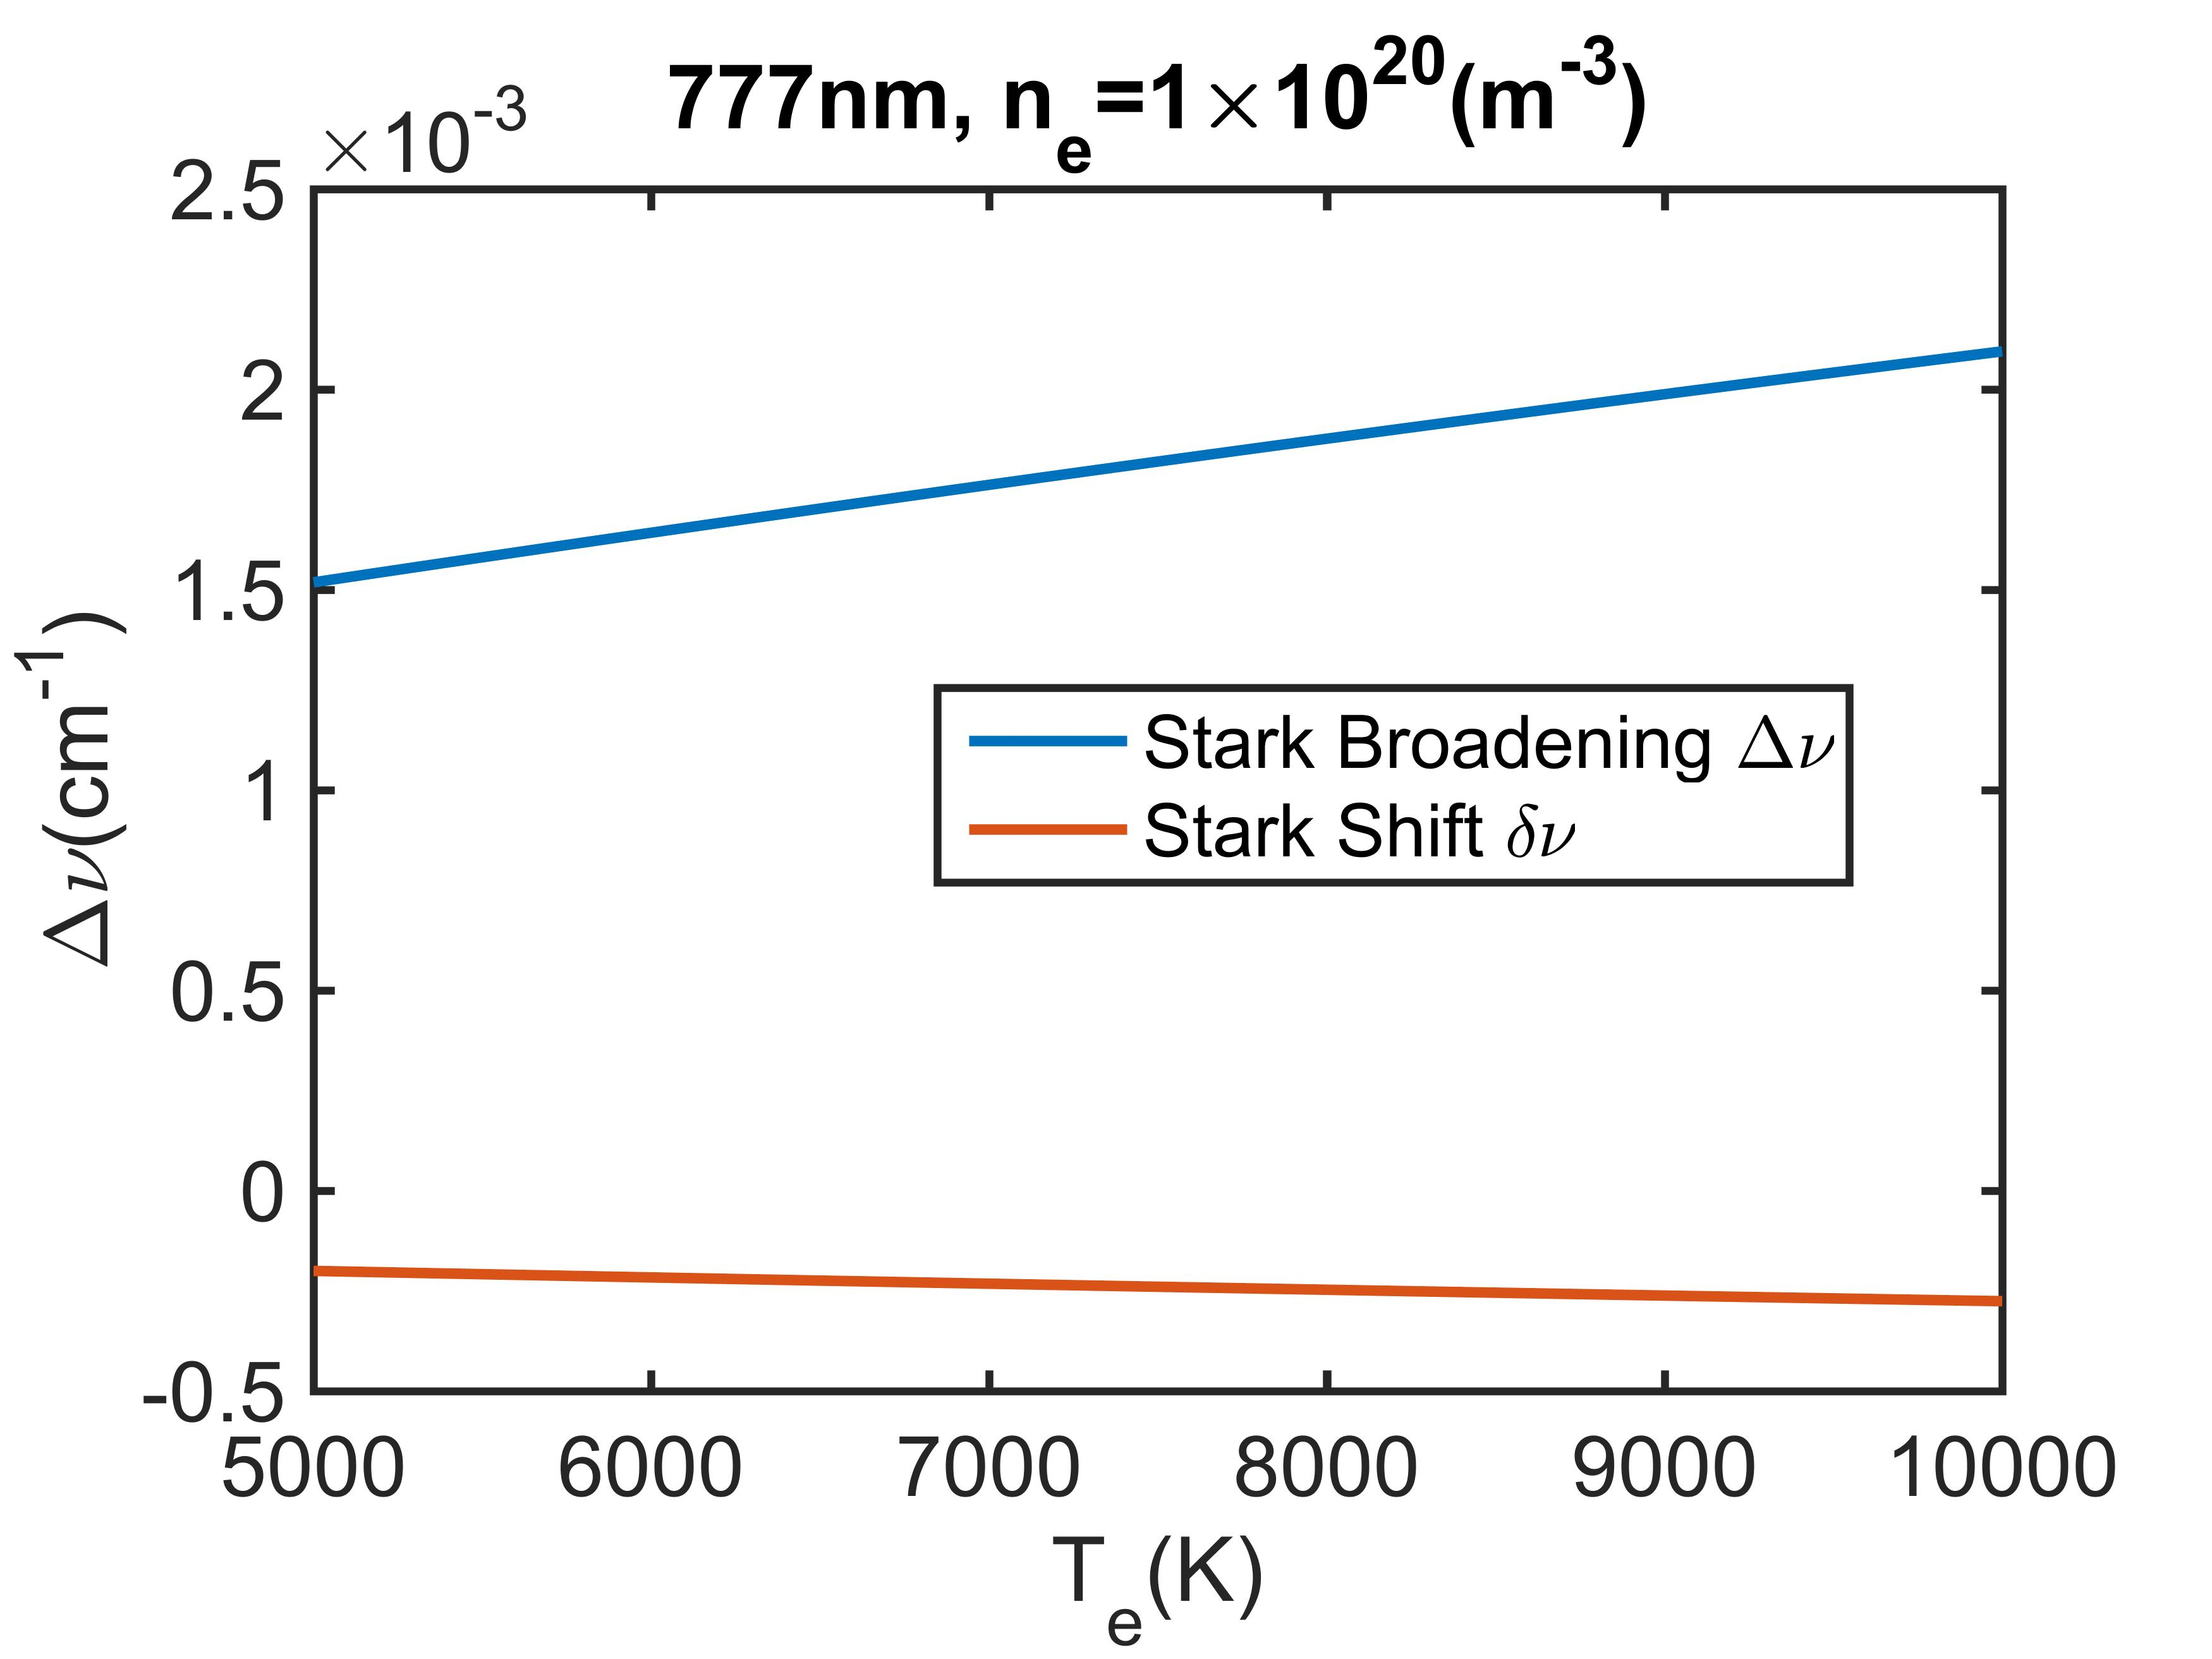
\includegraphics[width=\textwidth]{delta_vs_Tdependance_777.jpg}
      \caption{\label{fig:delta_vs_Tdependance_777} }
      \end{subfigure}
    \caption{\label{fig:delta_vs_Tdependance} Temperature dependence of the Stark effect at a constant electron number density. }
\end{figure}

In general, a discharge cell is needed to provide the reference wavelength center for the Stark shift measurement\cite{Baer1992c}. However, using the discharge cell to determine the reference wavelength center has two drawbacks: (1) the $n_e$ and the corresponding Stark shift in the discharge cell need to be calibrated beforehand; (2) The van der Waals shift in the sample gases needs to be accounted for, which is even more challenging than (1) because the van der Waals shift is usually poorly known. 

The current paper circumvented the need of a reference discharge cell by in-situ measurements of the Stark shift behind reflected shock waves. The line-center of the first scan with a reliable Voigt fit behind the reflected shock wave (usually within 50 $\mu$s) is used as the reference line-center position. It is assumed that within the first 50 $\mu$s after the passage of the reflected shock wave, electron number density is negligible due to the slow onset of Ar ionization (on the order of a few hundred $\mu$s determined by the ionization rates shown in the later section). Therefore the Stark shift is approximately zero for the first scan. Using the fitted line-center of the first scan as reference, the Stark shifts of the future scans are directly obtained from the relative line-center shift.  As discussed further in the uncertainty analysis section, the van der Waals shift drift in determining the Stark shift is negligible in the current measurements. The pressure is kept relatively constant throughout the test time using a driver insert, and therefore the van der Waals shift of the future scans caused by the pressure change could be neglected.

% The lineshape function we used in the 

\subsection{A simplified collisional-radiative model}
A simplified collisional-radiative model was developed previously in our lab to describe the collisional excitation kinetics of the atomic oxygen in argon bath gas (1\% O$_2$/Ar)\cite{Li2019_modeling}. The rate constants of the model were optimized by matching the population time history of O(3s $^5$S$^0$) measured by laser absorption spectroscopy. The model included 7 species: ground state molecular oxygen O$_2$, ground state atomic oxygen O($^3P$), the 4$^{th}$ energy level of atomic oxygen O(3s $^5$S$^0$), ionized atomic oxygen O$^+$, ground state argon Ar, ionized argon Ar$^+$, and electrons e$^-$. 

According to the previous model, the kinetics of the excited-state oxygen atoms were dominated by collisions with heavy particles (Ar) at the initial stage and collisions with electrons in the later stage. To match the measured O(3s $^5$S$^0$) population time histories, the electron and heavy particle impact ionization rates of Ar in this simplified model were adjusted $\sim$ 18 times larger than their nominal values in the literature, which were generally considered to be accurate within their reported uncertainty($\sim 20\%$). 

The current electron number density diagnostic can be used to validate the previous modeling results. As will be shown in the next section, the electron number density predicted by the model and measured from the current 926 nm transition Stark shift generally agree within a factor of 2, providing support for the model and its kinetics rate constants.

\section{Results}
A sample measurement of the pressure trace and the laser intensity are shown in Figure \ref{fig:rawI}. The raw laser intensity is converted to absorbance using equation \ref{eq:beer's_law}. The absorbance in the time domain is converted to the frequency domain using an etalon with FSR =0.0688 cm$^{-1}$. 

\begin{figure}[h]
    \centering
    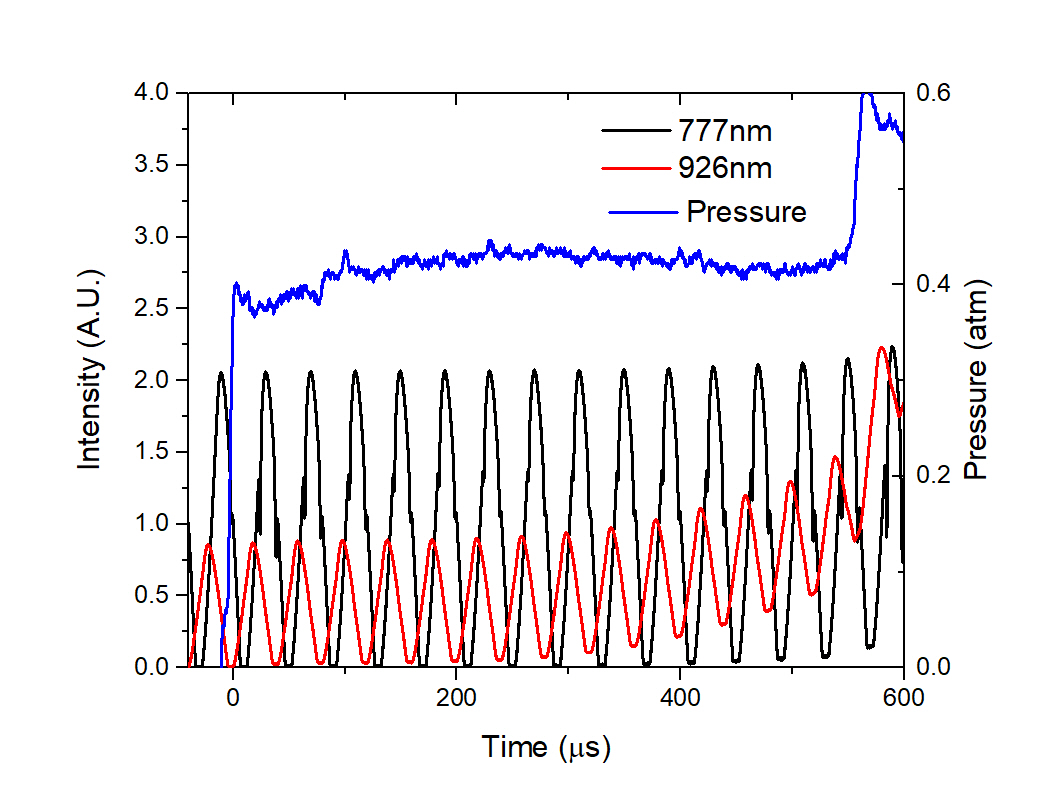
\includegraphics[width=0.6\textwidth]{rawI_24_40mil.jpg}
    \caption{The raw laser intensity on detector and the pressure trace.}
    \label{fig:rawI}
\end{figure}

\subsection{Lineshape Voigt fit}
\begin{figure}[h]
  \centering
    \begin{subfigure}[b]{0.4\textwidth}
     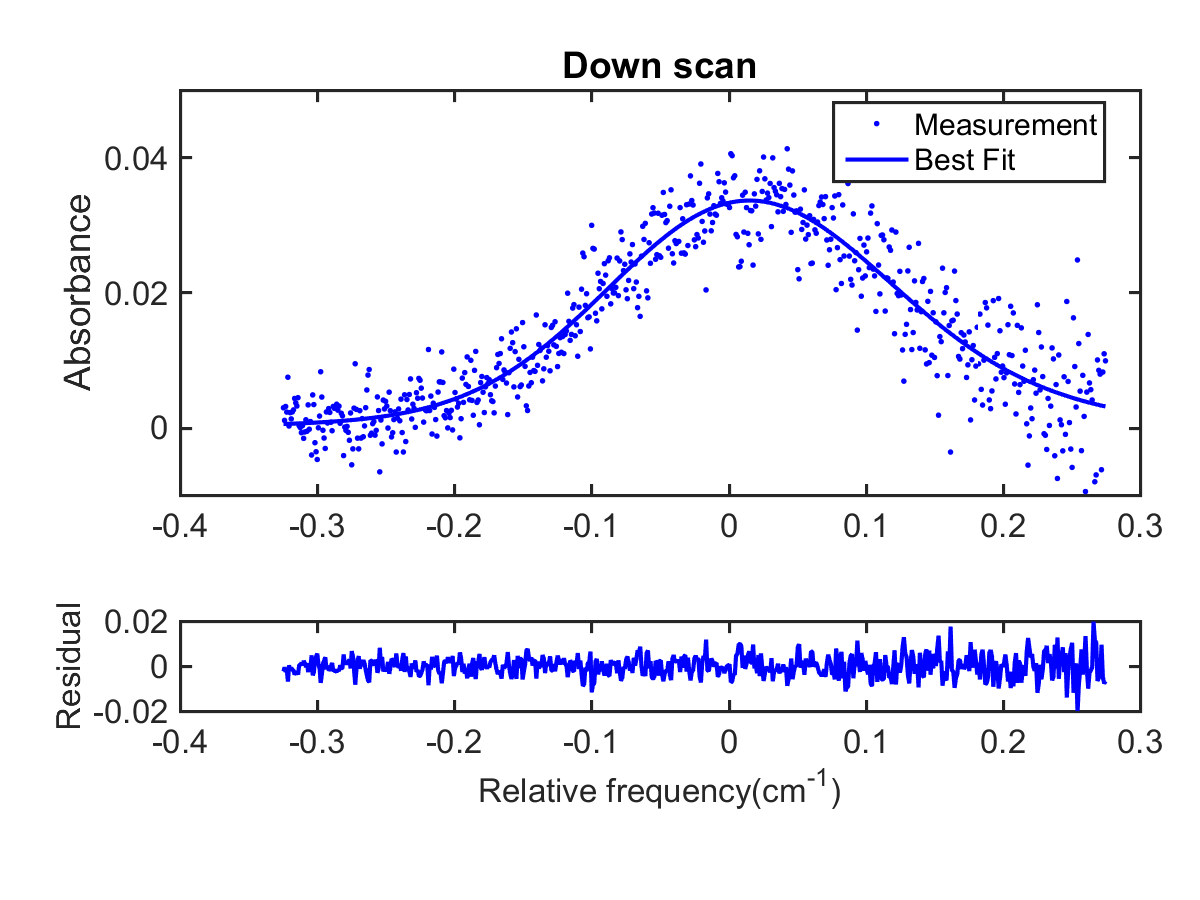
\includegraphics[width=\textwidth]{11209K_037atm_abs_down_one_scan_926.png}
    \caption{\label{fig:lineshape_fit_downScan_926} }   
      \end{subfigure} %
    \begin{subfigure}[b]{0.4\textwidth}
     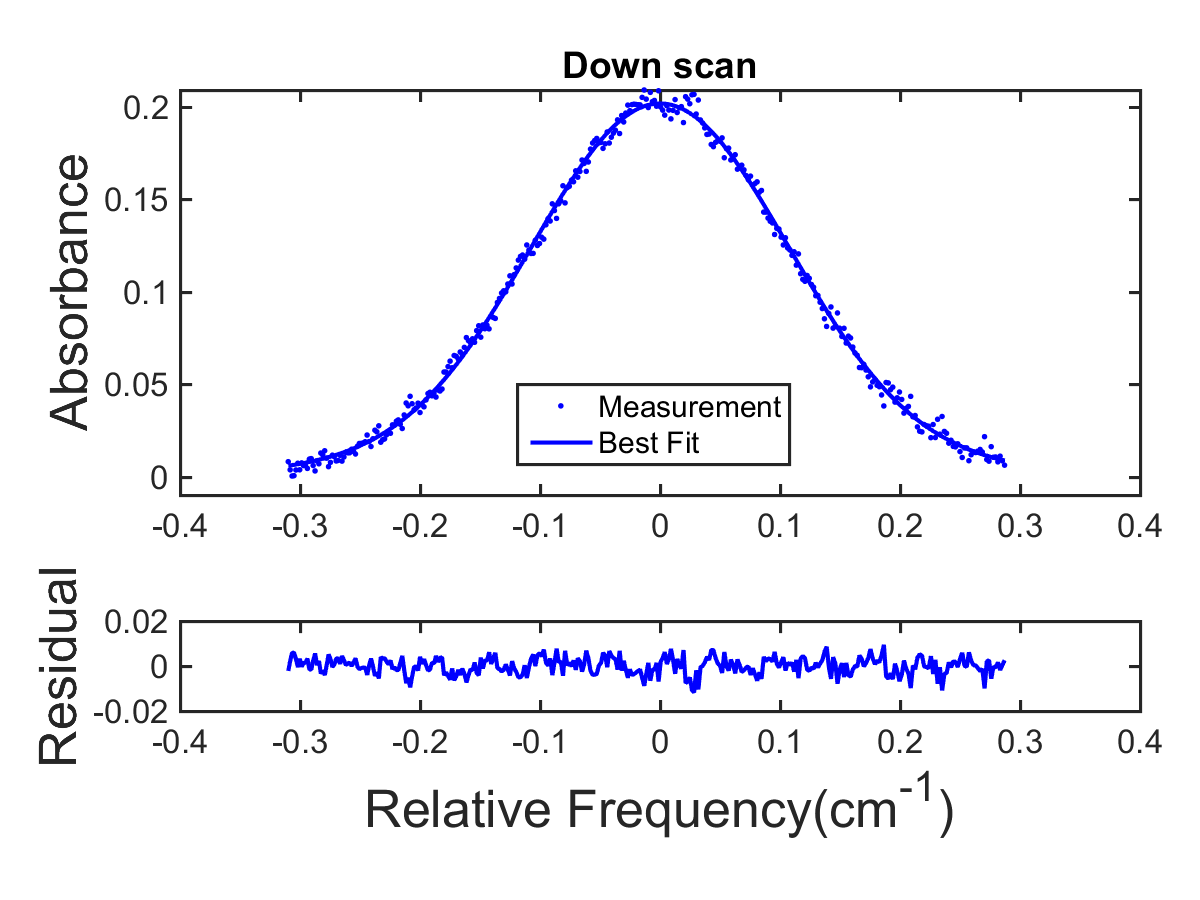
\includegraphics[width=\textwidth]{11209K_037atm_abs_down_one_scan.png}
    \caption{\label{fig:lineshape_fit_downScan_777} }   
      \end{subfigure} %
    \caption{\label{fig:lineshape_fit_777} Sample measurements of the absorbance and the best Voigt fit for (a) the 926 nm transition and (b) the 777 nm transition. T$_{5,0}$=11209K,P$_{5,0}$=0.37atm, t $\approx$ 200$\mu s$. The residual plots represent the absolute residuals for both transitions.}
\end{figure}
A sample measurement of the absorbance for the O(3p $^5$P$_{3}$) to O(3d $^5$D$_{2,3,4}^0$) transition and its best Voigt fit at $T_{5,0}=$11,209 K and $P_{5,0}$=0.37 atm is shown in figure \ref{fig:lineshape_fit_downScan_926}.  Similarly, the absorbance for the O(3s $^5$S$^0$) to O(3p $^5$P$_{3}$) transition at 777 nm  is shown in Figure \ref{fig:lineshape_fit_downScan_777}. The initial translational temperature immediately after the reflected shock passed by, $T_{5,0}$, is calculated from FROSH before O$_2$ dissociates assuming vibrational equilibrium. The residual amplitude is approximately 0.01 for both transitions, but the peak absorbance for the 777 nm transition is approximately five times larger than that of the 926 nm transition because of the larger population of the O(3s $^5$S$^0$) state than the O(3p $^5$P$_{3}$) state. Despite the lower SNR, the Stark shift of the 926 nm transition is more sensitive as an electron number density diagnostic because of the large Stark parameters $w,d$, as shown below. 

The low SNR for the 926 nm transition restricted our detection limit to  conditions of T$_{5,0}>$10,000 K and $n_e>1\times10^{20}$m$^{-3}$. Note that these limitations can be extended if the O(3p $^5$P$_{3}$) population is in chemical equilibrium because the SNR would be an order of magnitude better. The current measurements show that the O(3p $^5$P$_{3}$) population is generally an order of magnitude lower than its Boltzmann equilibrium value calculated at the translational temperature. Another way to improve the SNR is to use cavity-enhanced absorption spectroscopy\cite{nations2015_new,sun_kai_2014,Chao2019}.   

The measured absorbance was fitted with a Voigt lineshape using equation \ref{eq:beer's_law}. The absorbance of the 777 nm transition from the 4$^{th}$ energy level (O(3s $^5$S$^0$)) to the 6$^{th}$ energy level(O(3p $^5$P$_{3}$)) is fitted by $\alpha_{4}(\nu) = S_{46}n_4L\phi_{V}(\Delta \nu^{(4)}_c,\Delta \nu^{(4)}_d, \nu_0^{(4)})$, where $S_{46}$ is the line strength of the transition from level 4 to 6, $n_4$ is the population of level 4, $L$ is the optical path length, $\phi_{V}(\Delta \nu^{(4)}_c,\Delta \nu^{(4)}_d, \nu_0^{(4)})$ is the Voigt lineshape with line-center $\nu_0^{(4)}$, collisional broadening $\Delta \nu_c^{(4)}$, Doppler broadening $\Delta \nu_d^{(4)}$. The absorbance of the 926 nm transition from the 6$^{th}$ energy level to the 10$^{th}$ energy level(O(3d $^5$D$_{2,3,4}^0$)) is fitted by $\alpha_{6}(\nu) = n_6L\sum_j S^j_{6,10}\phi^j_{V}(\Delta \nu^{(6)}_{c,j},\Delta \nu^{(6)}_{d,j}, \nu_{0,j}^{(6)})$, where $j=1, 2, 3$ runs through the upper level J=2, 3, 4. For simplicity, we assume that the Stark shifts and the collisional broadening widths for the three blended lines of the 926 nm transition are same. The line-center frequency $\nu^{(6)}_{0,j}$ is taken from the NIST database.  


\begin{figure}[h]
  \centering
    \begin{subfigure}[b]{0.45\textwidth}
     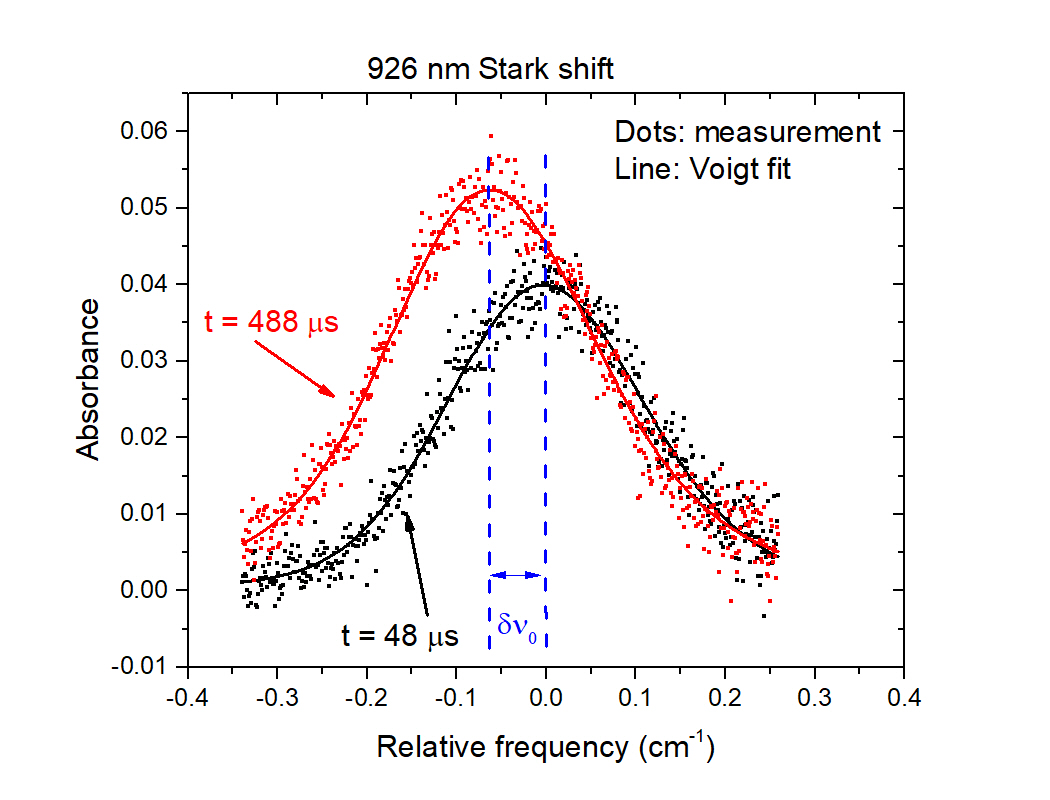
\includegraphics[width=\textwidth]{lineshape_time_history_concise_926.jpg}
    \caption{\label{fig:lineshape_shift_time_history}}  
      \end{subfigure} %
    \begin{subfigure}[b]{0.45\textwidth}
     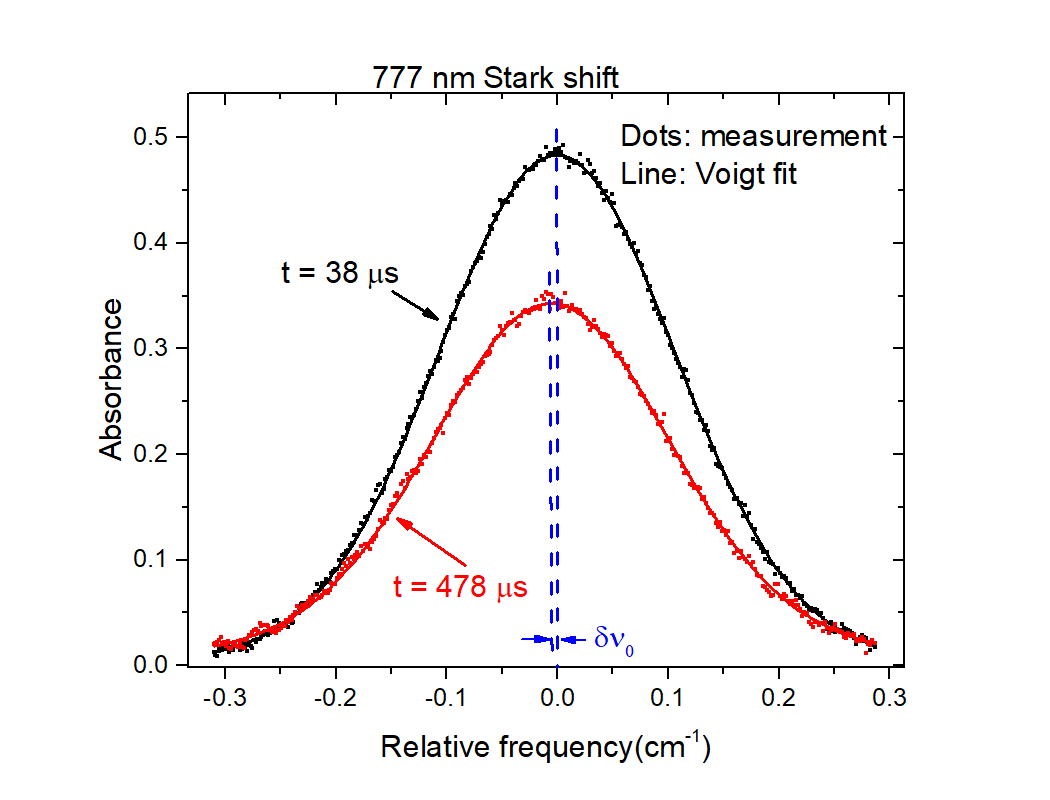
\includegraphics[width=\textwidth]{lineshape_time_history_concise_777.jpg}
      \caption{\label{fig:lineshape_shift_time_history_777} }
      \end{subfigure}
    \caption{\label{fig:lineshape_shift_time_history_777_926} (a) 926 nm absorbance at 48 $\mu$s and 488 $\mu$s. The Stark shift of the line-center is approximately $\delta_{\nu_0}=$-0.06 cm$^{-1}$. (b) 777 nm absorbance at 48 $\mu$s and 488 $\mu$s. The Stark shift of the line-center is approximately $\delta_{\nu_0}=$-0.005 cm$^{-1}$. }
\end{figure}
The best Voigt fit of the absorbance  was found using the Matlab function ``lsqcurvefit". The corresponding collisional broadening, Doppler broadening, and line-center($\Delta \nu_c,\Delta \nu_d$, and $\nu_0$) and their fitting uncertainties are obtained from the best Voigt fit. The 926 nm absorbance at t = 48 and 488 $\mu$s are plotted in figure \ref{fig:lineshape_shift_time_history}. The absorbance spectrum at t = 48 $\mu$s is used as the reference wavelength center to determine the Stark shifts for future scans, with the assumption that a negligible amount of electrons are formed within the first $50 \mu$s. This assumption is justified by the measurements and simulations shown in the next section.Figure \ref{fig:lineshape_shift_time_history} shows at t= 488 $\mu$s, the Stark shift is approximately -0.06 cm$^{-1}$. On the other hand, the Stark shift of the 777 nm transition is approximately -0.005cm$^{-1}$ as shown in figure \ref{fig:lineshape_shift_time_history_777}. Such small Stark shifts make the measurement subject to noise.

\begin{figure}[h]
  \centering
    \begin{subfigure}[b]{0.45\textwidth}
     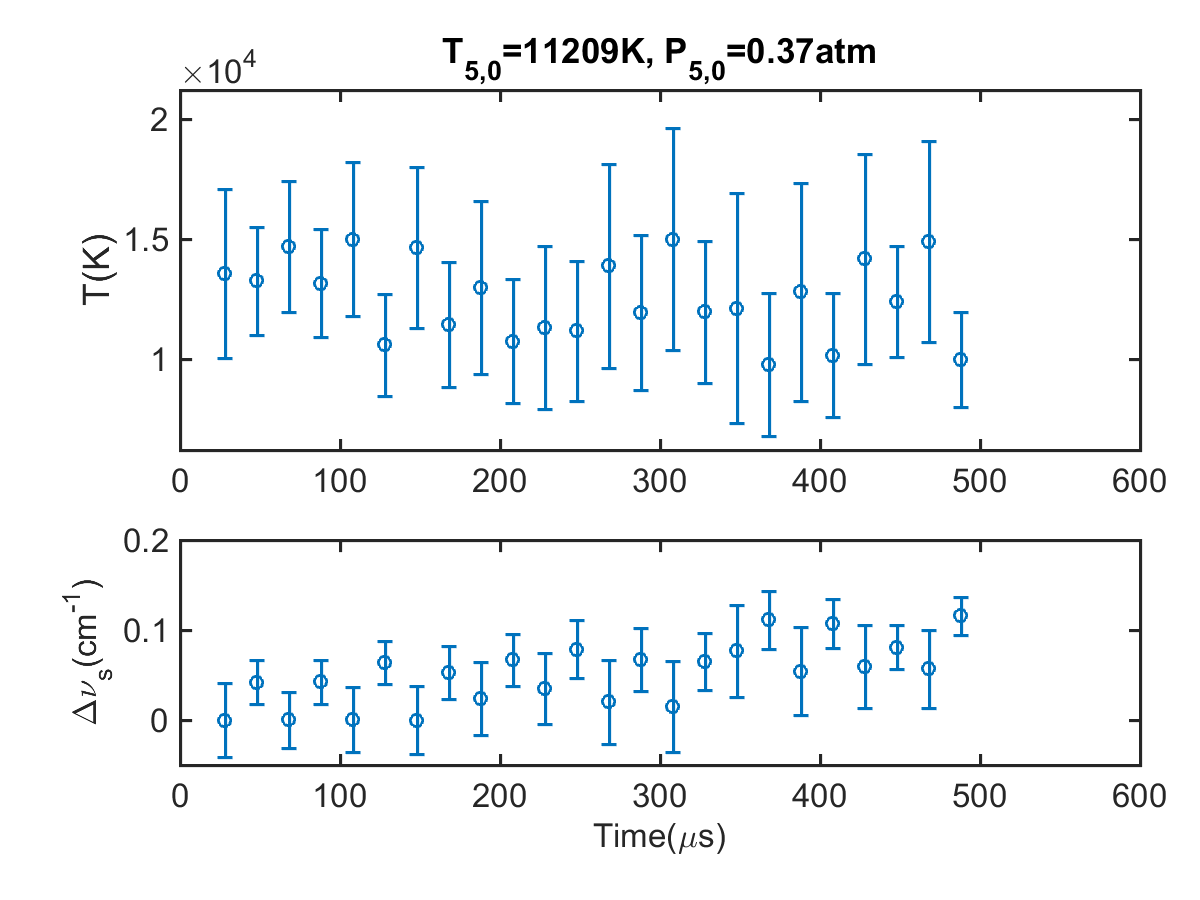
\includegraphics[width=\textwidth]{11209K_037atm_T_vs_926.png}
    \caption{\label{fig:Tdoppler}}  
      \end{subfigure} %
    \begin{subfigure}[b]{0.45\textwidth}
     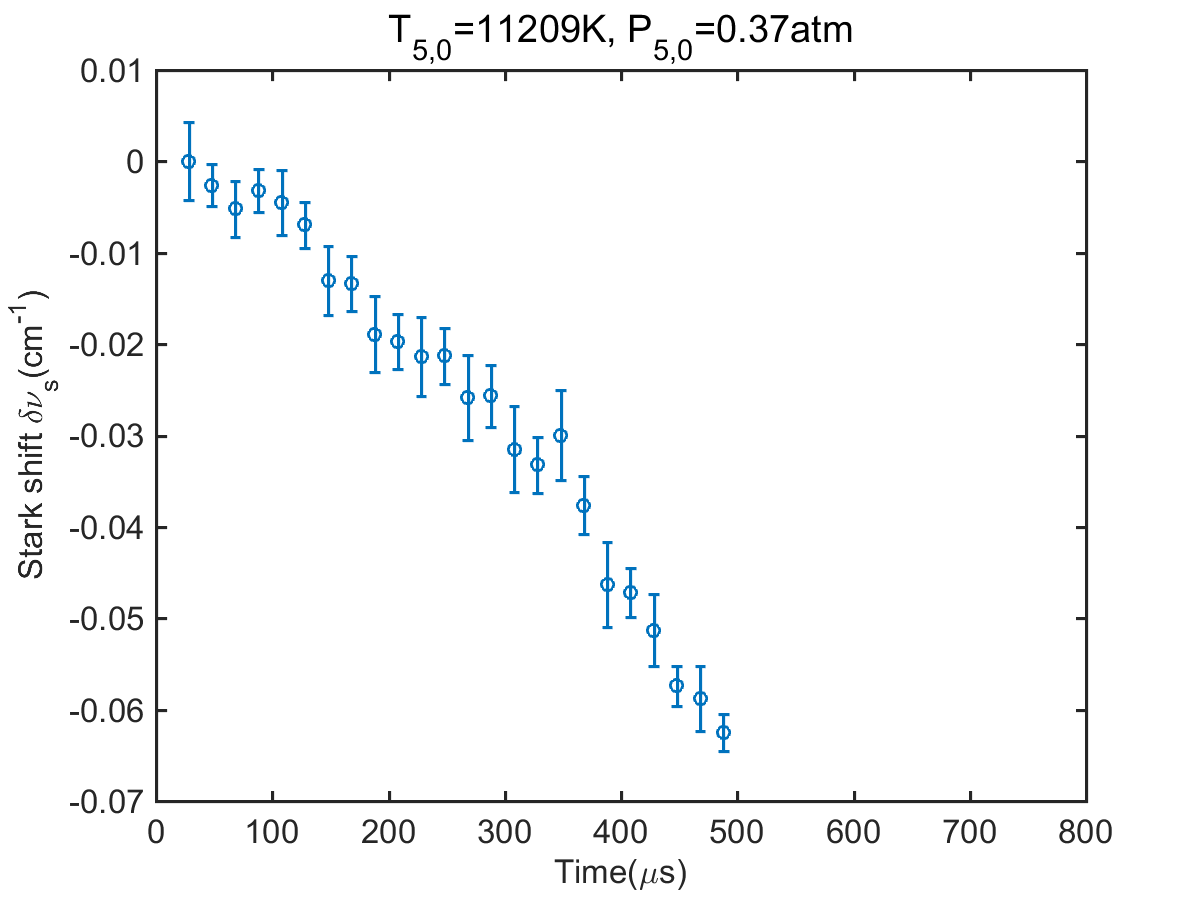
\includegraphics[width=\textwidth]{11209K_037atm_stark_shift_926.png}
      \caption{\label{fig:stark_shift_time_history} }
      \end{subfigure}
    \caption{\label{fig:broadening_and_shift} (a) Temperature $T(t)$ and Stark broadening $\Delta\nu_s(t)$ calculated from the best-fit Doppler width and collisional width of the 926 nm transition. (b) The Stark shift $\delta\nu_s(t)$ calculated from the relative line-center shift. The Stark shift per measurement period is approximately -0.0024cm$^{-1}$/20$\mu$s. Error bars represent the uncertainty of lineshape fit. }
\end{figure}
The Doppler broadening and the Stark broadening from the best Voigt fit are shown in Figure \ref{fig:Tdoppler}.  Error bars represent the uncertainty of lineshape fit, which are calculated from the 95\% confidence interval of the Voigt fit. $T(t)$ is inferred from the Doppler width using equation \ref{eq:doppler_width} and $\Delta\nu_s(t)$ is calculated by subtracting the the van der Waals FWHM of the first reliable scan from the total collisional widths. Because of the large scatter and obvious oscillation based on the scanning direction of $\Delta \nu_s(t)$, the 926 nm Stark broadening could not be used to infer $n_e$ reliably. The large scatter in $T(t)$ and  $\Delta\nu_s(t)$ is caused by the low SNR of the 926 nm transition and the difficulty to accurately fit linewidth as explained before. Figure \ref{fig:stark_shift_time_history} shows that the Stark shift fit is more robust than the linewidth fit in figure \ref{fig:Tdoppler}, as manifest by the less-scattered data and smaller relative error bars compared with those in $T(t)$ and  $\Delta\nu_s(t)$. The Stark shift within the test time is measured to be approximately -0.06 cm$^{-1}$/500$\mu$s, corresponding to a time resolution of -0.0024cm$^{-1}$/20$\mu$s for the current $n_e$ diagnostic.
 
\begin{figure}[h]
  \centering
    \begin{subfigure}[b]{0.45\textwidth}
     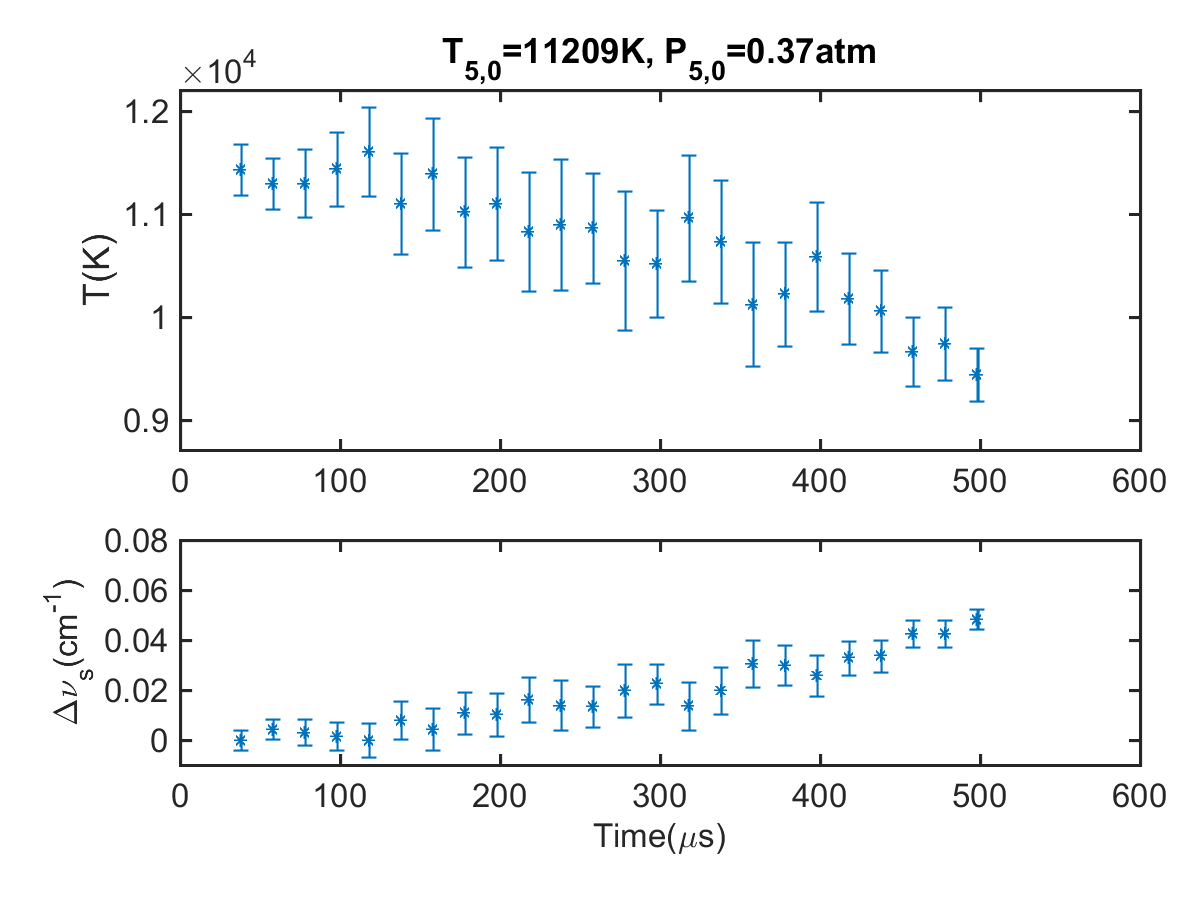
\includegraphics[width=\textwidth]{11209K_037atm_T_vs_777.png}
    \caption{\label{fig:Tdoppler_vs_777}}  
      \end{subfigure} %
    \begin{subfigure}[b]{0.45\textwidth}
     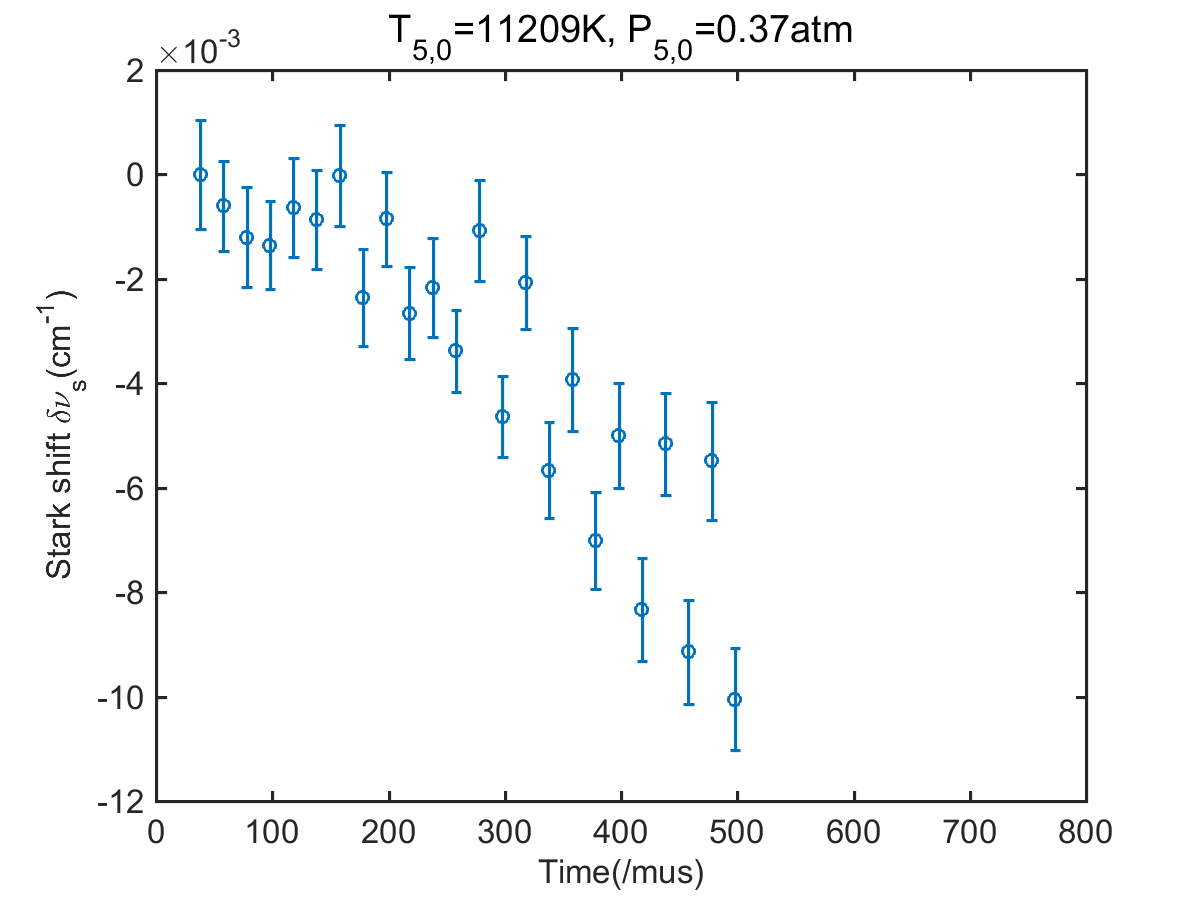
\includegraphics[width=\textwidth]{11209K_037atm_stark_shift_777.png}
      \caption{\label{fig:stark_shift_time_history_777} }
      \end{subfigure}
    \caption{\label{fig:broadening_and_shift_777} (a)  Temperature $T(t)$ and Stark broadening $\Delta\nu_s(t)$  calculated from the best-fit Doppler width and collisional width of the 777 nm transition. (b) The Stark shift $\delta\nu_s(t)$ calculated from the relative line-center shift. Error bars represent the uncertainty of lineshape fit.}
\end{figure}
Figure \ref{fig:broadening_and_shift_777} shows the linewidth and line-center fit for the 777 nm absorbance  in comparison for figure \ref{fig:broadening_and_shift}. The linewidth fitting shows smaller scatter and oscillation due to the better SNR of the 777 nm absorbance. The line-center shift is subject to noise because of the small amplitude of the Stark shift compared with figure \ref{fig:stark_shift_time_history}. The 777 nm Stark broadening/shift are less sensitive to $n_e$ because of the small $w,d$ parameters in Table \ref{tab:Stark_parameters}. The $n_e$ results inferred from the 777 and 926 nm absorbance are discussed in the next section.



\subsection{Inferred electron number density time history}
In principle, there are four ways to infer the electron number density in the current study, using either the Stark broadening or shift, and for either the 777 or 926 nm absorbance lineshapes. Among these four diagnostics, the 926 nm Stark shift is the most sensitive and robust as shown below.


\begin{figure}[h]
    \centering
    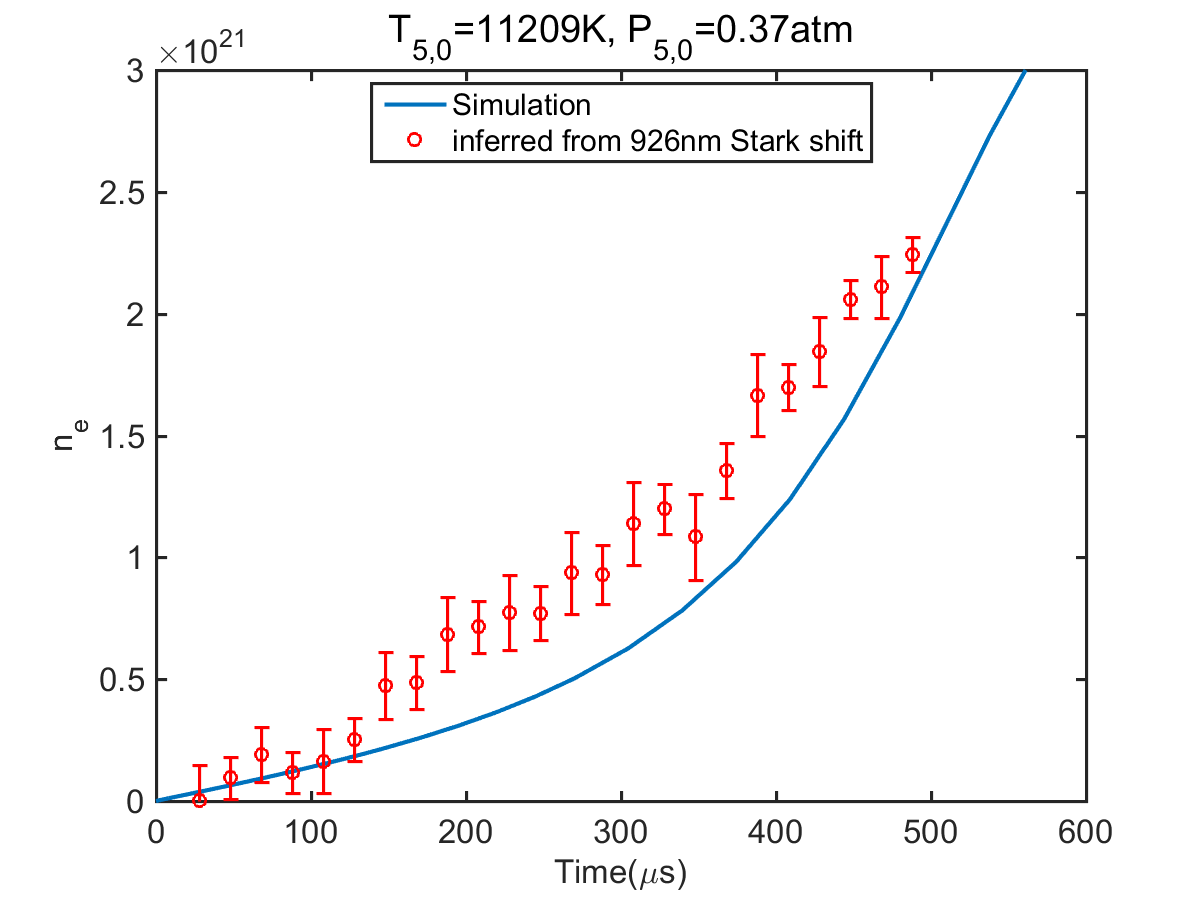
\includegraphics[width=0.6\textwidth]{11209K_037atm_ne_sim_926.png}
    \caption{Symbols: $n_e(t)$ inferred from the 926 nm Stark shift in figure \ref{fig:stark_shift_time_history}.  Error bars represent the uncertainty of lineshape fit. Line: $n_e(t)$ predicted by the previously developed model. }
    \label{fig:ne_time_history}
\end{figure}
In figure \ref{fig:ne_time_history}, the electron number density is calculated from the 926 nm Stark shift in figure \ref{fig:stark_shift_time_history} using equation \ref{eq:stark_shift}. The uncertainty of the electron number density is propagated from that of the fitted Stark shift by numerically calculated gradient using equation \ref{eq:stark_shift}. The electron number density increases from 0 immediately after the reflected shock to $2.5\times10^{21}$ m$^{-3}$ within the 520$\mu s$ test time. The measured and simulated electron number density generally agree with each other within the test time, which provides confidence in both the diagnostic method and the model, although they may suffer from uncertainties of the Stark shift parameter and the bias of the model.

In the previous model\cite{Li2019_modeling}, the heavy particle and electron impact ionization rates for Ar were adjusted to be $\sim$ 18 times larger than their nominal values in the literature to match the O(3s $^5$S$^0$) population time history measurements.  This fast electron formation rate is validated by the current electron number density diagnostics. It is likely caused by the model under-estimation of the electron formation due to the lack of reliable oxygen ionization rates, over-simplification of the kinetic model and systematic experimental effects such as impurities in the shock tube. 

\begin{figure*}[h]
  \centering
  \begin{subfigure}[b]{0.4\textwidth}
     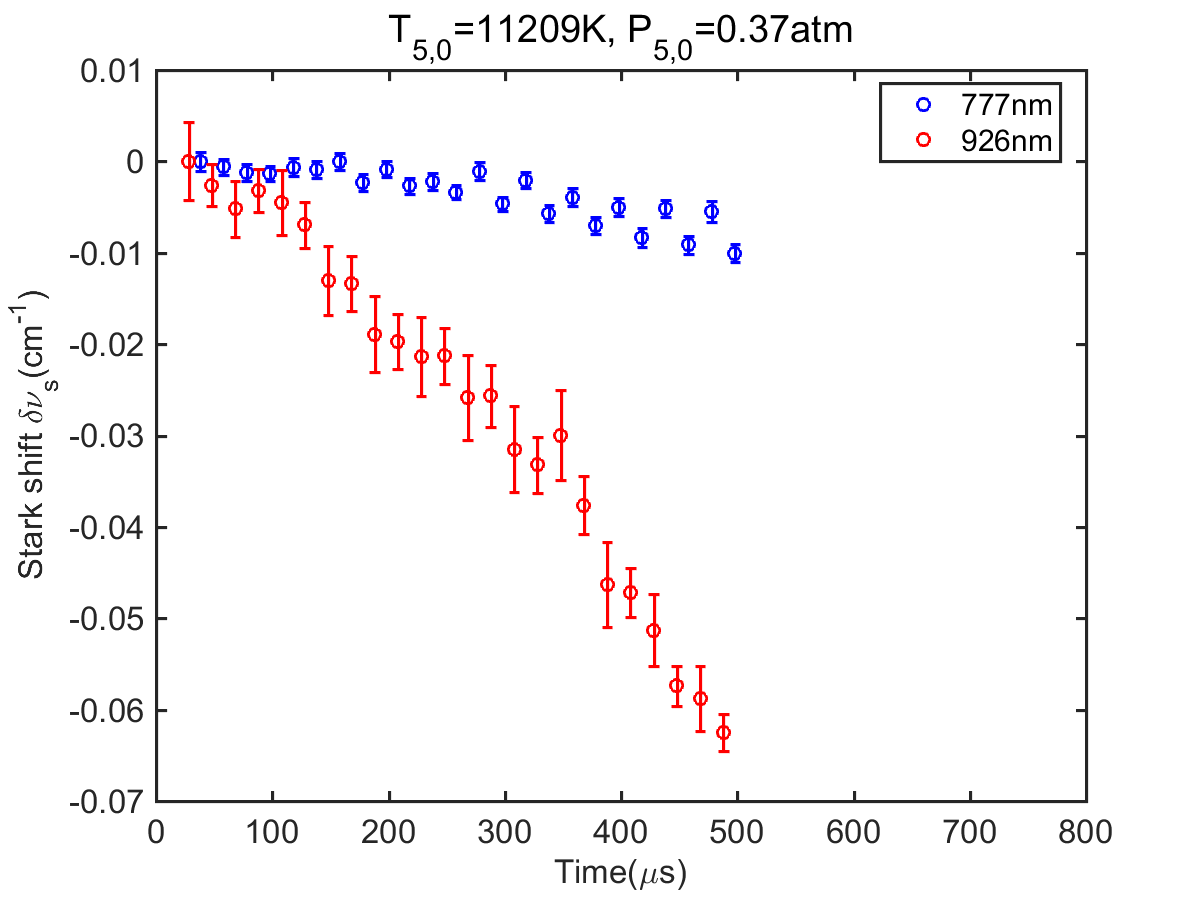
\includegraphics[width=\textwidth]{11209K_037atm_Stark_shift.png}
    \caption{\label{fig:stark_shift_777_926} }
    \end{subfigure}
    \begin{subfigure}[b]{0.4\textwidth}
         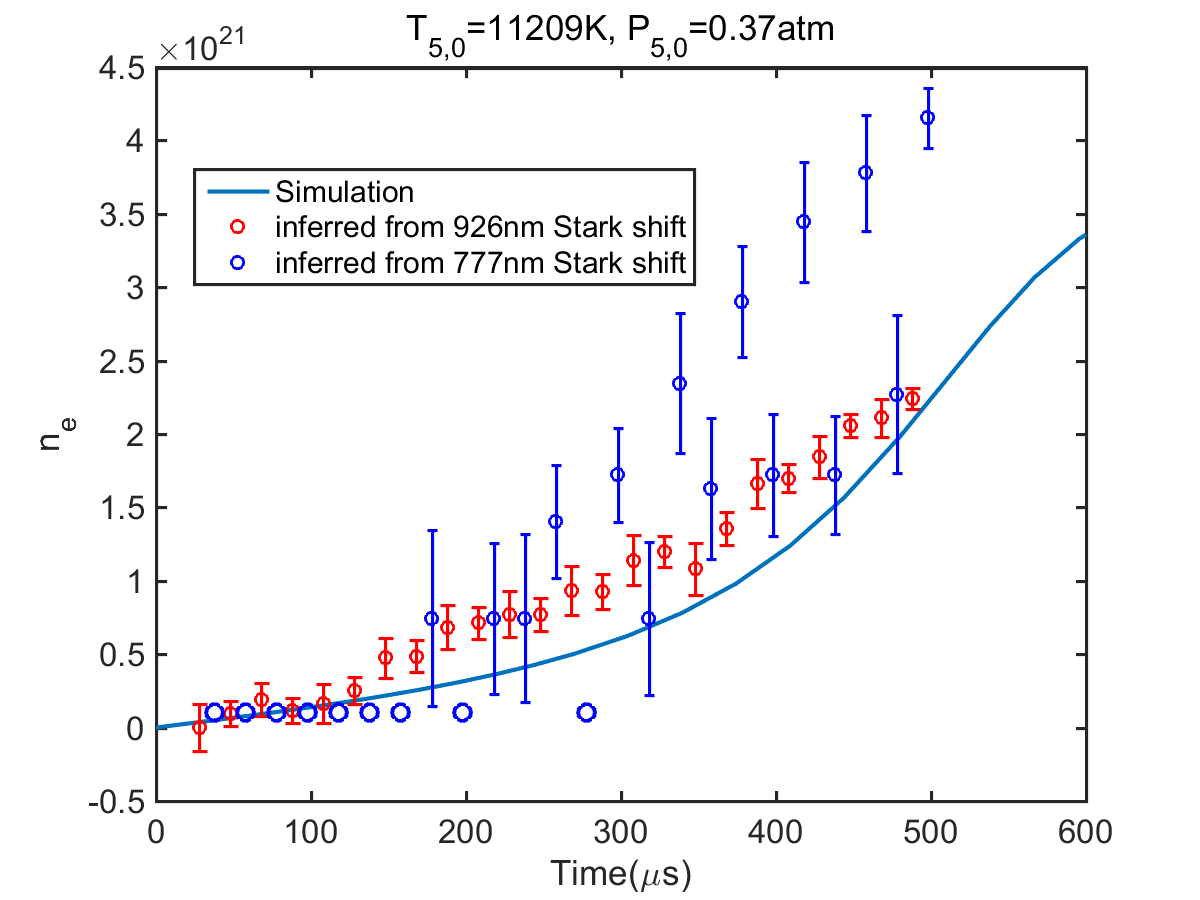
\includegraphics[width=\textwidth]{11209K_037atm_ne_sim_777_926.png}
    \caption{\label{fig:ne_777_926} }
   \end{subfigure}   
       \caption{\label{fig:compare_777_926} (a) Comparison of the 926 nm Stark shift in figure \ref{fig:stark_shift_time_history} with the 777 nm Stark shift. (b) $n_e(t)$ inferred from 777 nm and 926 nm Stark shifts.  Error bars represent the uncertainty of lineshape fit.}
\end{figure*}
Figure \ref{fig:stark_shift_777_926} combines the Stark shift time histories of the 777 and 926 nm absorbance in figure \ref{fig:stark_shift_time_history} and \ref{fig:stark_shift_time_history_777}. The 777 nm Stark shift is approximately an order of magnitude smaller than that of the 926 nm, as expected from Table \ref{tab:Stark_parameters}. The larger Stark shift of the 926 nm transition makes it more sensitive to $n_e$ and robust to noise compared with the 777 nm transition. Figure \ref{fig:ne_777_926} compares the electron number density inferred from the two Stark shifts in figure \ref{fig:stark_shift_777_926}. The overall general agreement in $n_e(t)$ based on the Stark shifts of the two transitions provides support in the Stark parameters in Table \ref{tab:Stark_parameters}. Note that the fitting uncertainty of $n_e(t)$ inferred from the 777 nm Stark shift is large and the error bars of adjacent values barely overlap; also some of the results hit the lower bound of the fit because the small Stark shift magnitude makes it very sensitive to noise. 

\begin{figure}
    \centering
    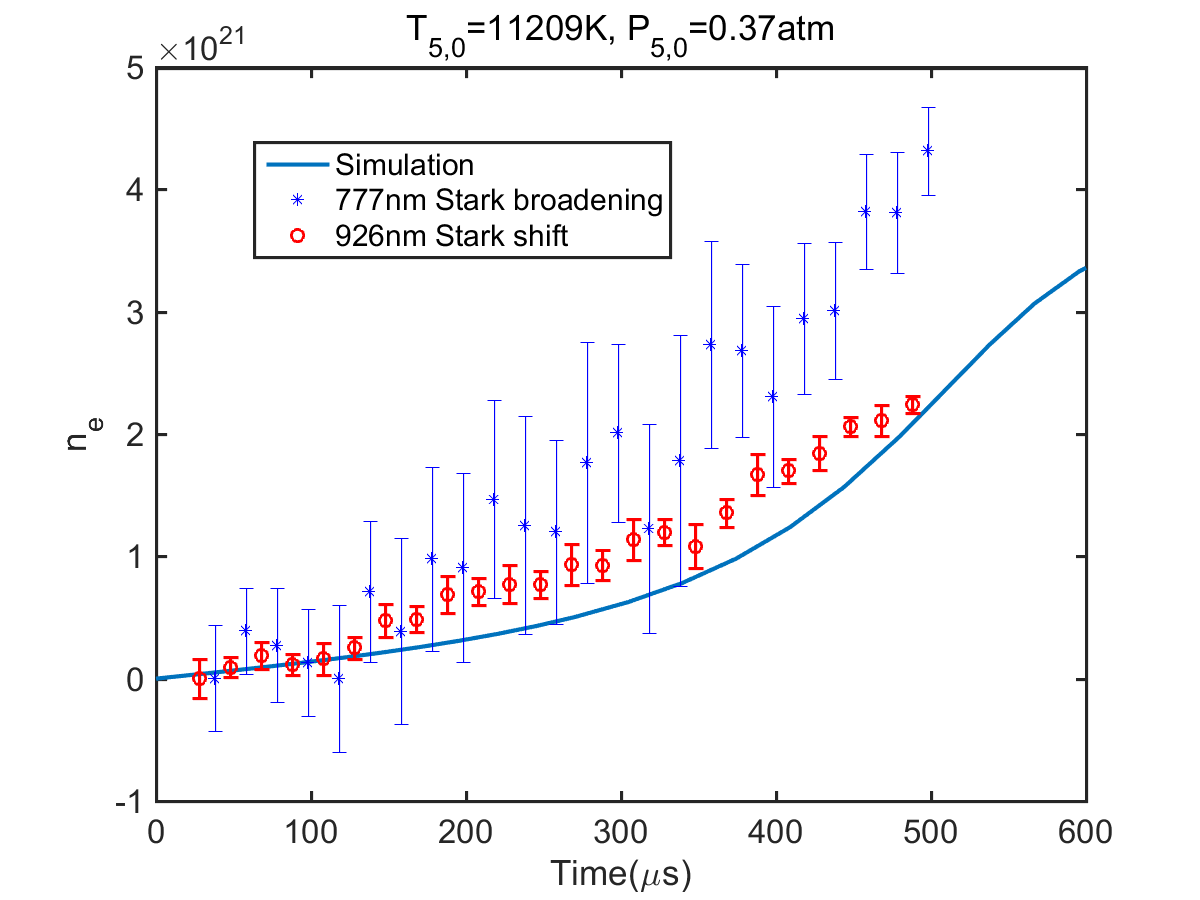
\includegraphics[width = 0.6\textwidth]{11209K_037atm_ne_sim_777Broadening_926.png}
    \caption{Comparison of $n_e(t)$ inferred from 777 nm Stark broadening and 926 nm Stark shift.  Error bars represent the uncertainty of lineshape fit.  The 777 nm $n_e$ uncertainty is larger than that of 926 nm because the uncertainty of linewidth fitting is larger than line-center fitting in general.  \label{fig:ne_777broadening_926}}
\end{figure}
As discussed in the introduction, the line-center fitting is generally more robust than linewidth fitting, which involves the convolution of various broadening mechanisms such as Doppler, Stark and van der Waals broadening.  Although it is not  always easy to reliably fit linewidth from the absorbance, it is possible to extract the 777 nm Stark broadening width for some high temperature cases, where the SNR is good. Hence $n_e(t)$ can be calculated from the 777 nm Stark broadening using equation \ref{eq:stark_broadening} and compared with that calculated from the 926 nm Stark shift. 

Figure \ref{fig:ne_777broadening_926} presents such a case, showing that the $n_e(t)$ calculated from the 777 nm Stark broadening and the 926 nm Stark shift agree approximately within the fitting uncertainty.  Note that the absolute uncertainty of the diagnostic methods is larger than the fitting uncertainties reported in figure \ref{fig:ne_777broadening_926}.  Again, the $n_e(t)$ agreement between different diagnostic methods gives us some confidence in the diagnostics themselves and the Stark parameters in Table \ref{tab:Stark_parameters}. Because of the large Stark parameters $w, \frac{d}{w}$, the electron number density calculated from the 926 nm Stark shift shows less scatter despite the lower SNR. 

More $n_e(t)$ measurements inferred from the 926 nm Stark shift in the range over 10,100 - 11,210 K are shown in figure \ref{fig:more_ne} together with the kinetic model predictions. The measurements generally agree with the model prediction within a factor of 2. Of course the current $n_e(t)$ data could be used to improve the kinetics model, as will be reported in a future paper.
\begin{figure}[h]
  \centering
    \begin{subfigure}[b]{0.4\textwidth}
     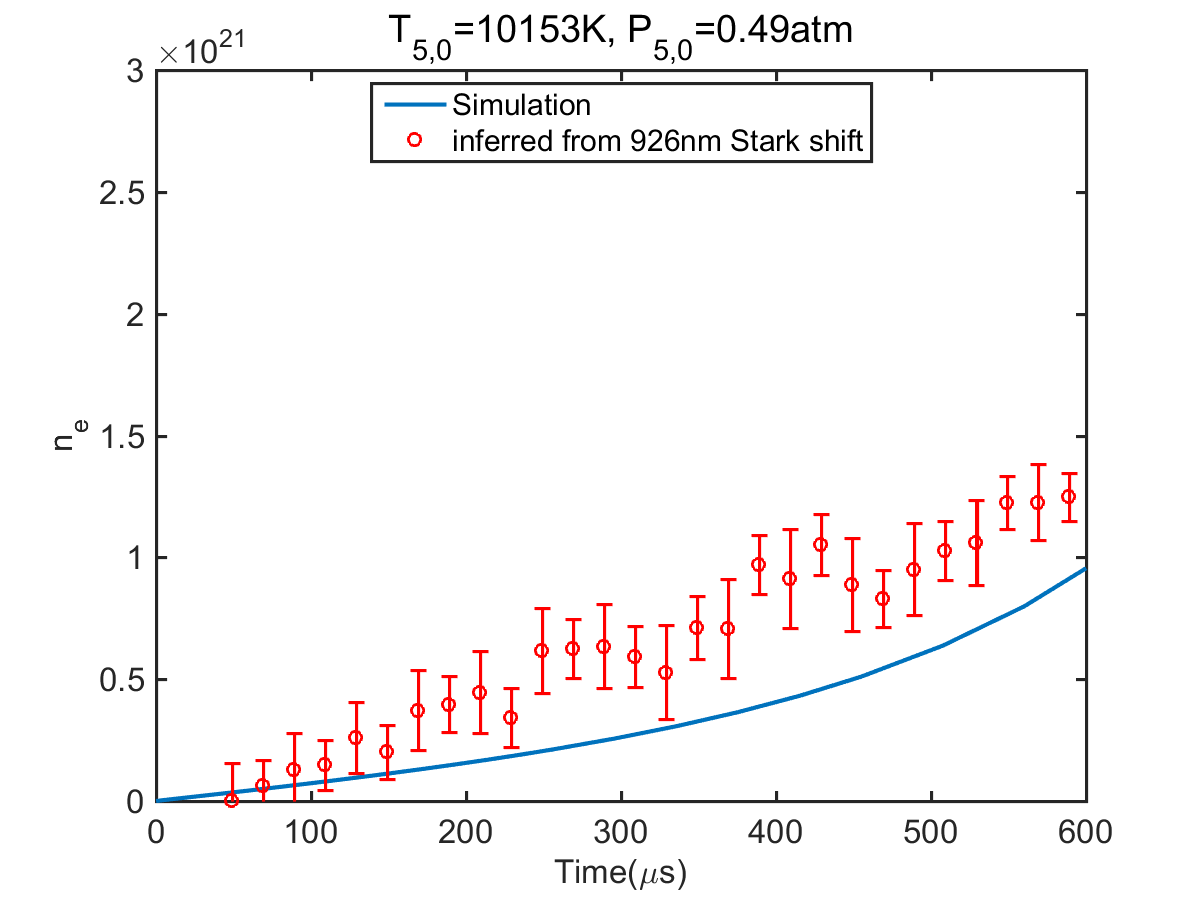
\includegraphics[width=\textwidth]{10153K_049atm_ne_sim_926.png}
    \caption{\label{fig:} }
      \end{subfigure} %
      \begin{subfigure}[b]{0.4\textwidth}
     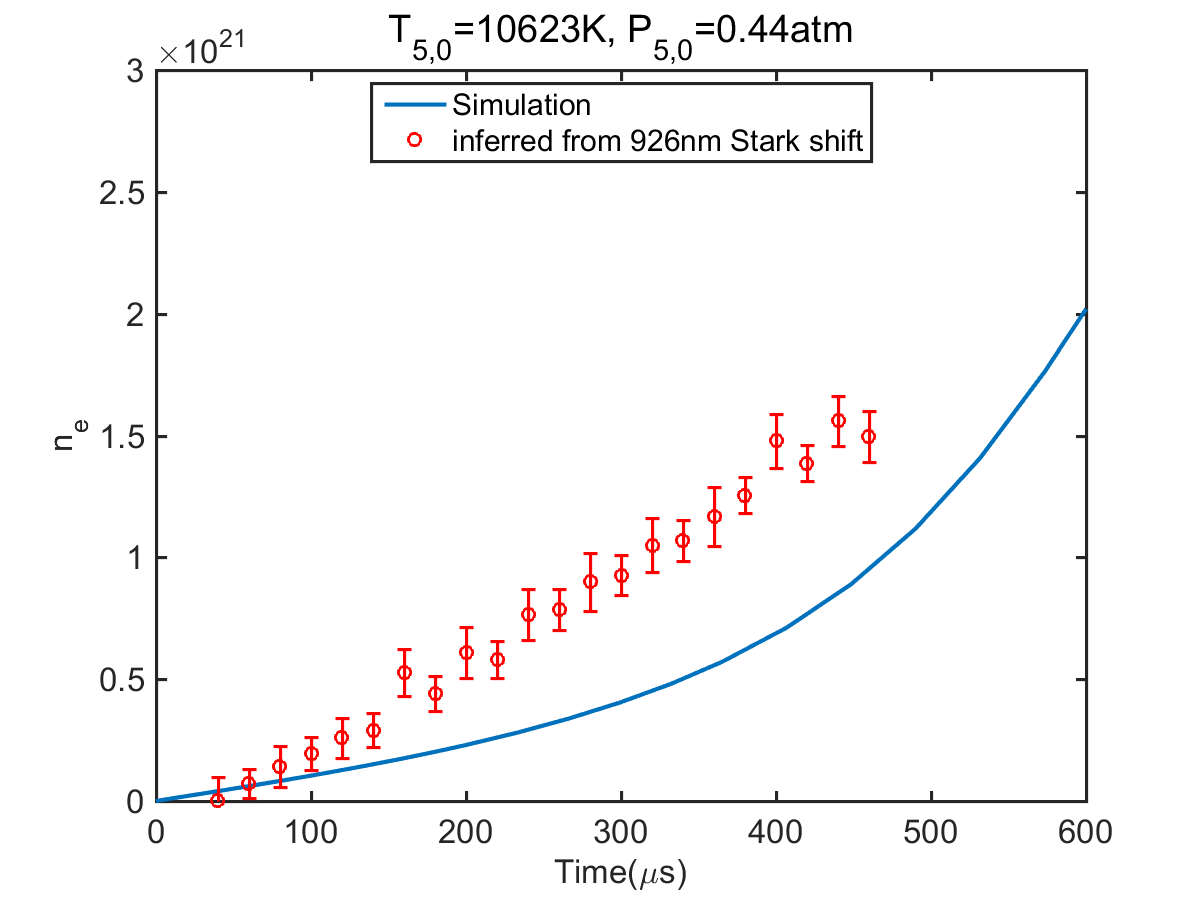
\includegraphics[width=\textwidth]{10623K_044atm_ne_sim_926.png}
      \caption{\label{fig:} }
      \end{subfigure}
    \begin{subfigure}[b]{0.4\textwidth}
     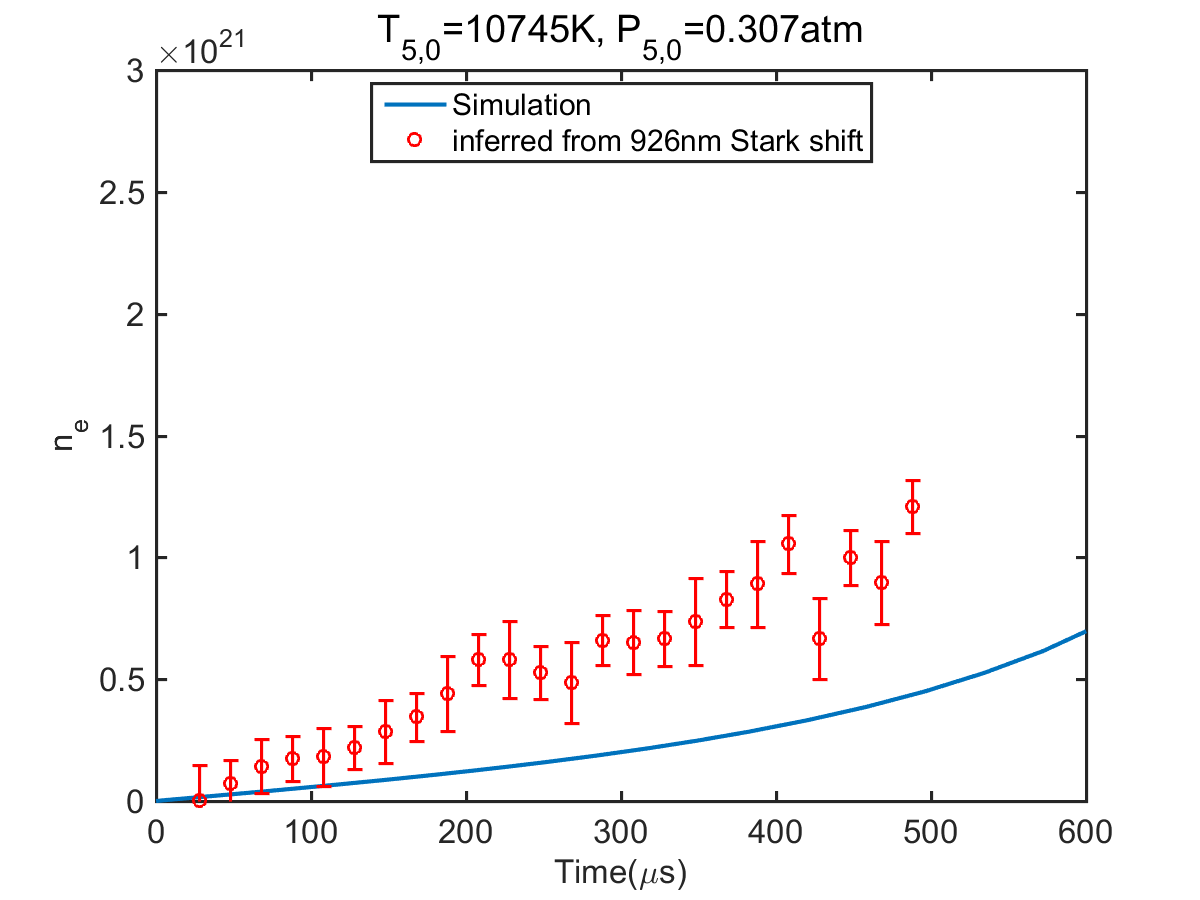
\includegraphics[width=\textwidth]{10745K_0307atm_ne_sim_926.png}
      \caption{\label{fig:} }
      \end{subfigure}
          \begin{subfigure}[b]{0.4\textwidth}
     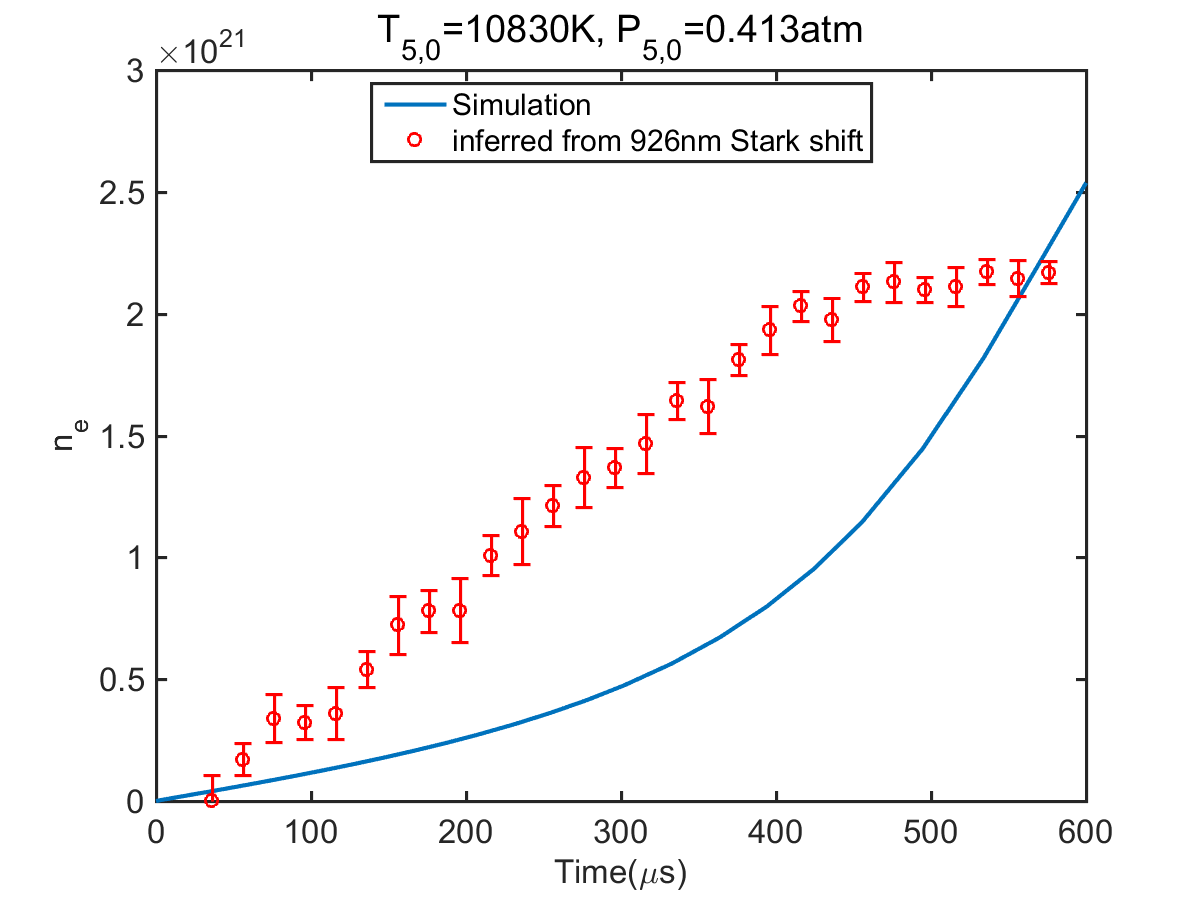
\includegraphics[width=\textwidth]{10830K_0413atm_ne_sim_926.png}
      \caption{\label{fig:} }
      \end{subfigure}
          \begin{subfigure}[b]{0.4\textwidth}
     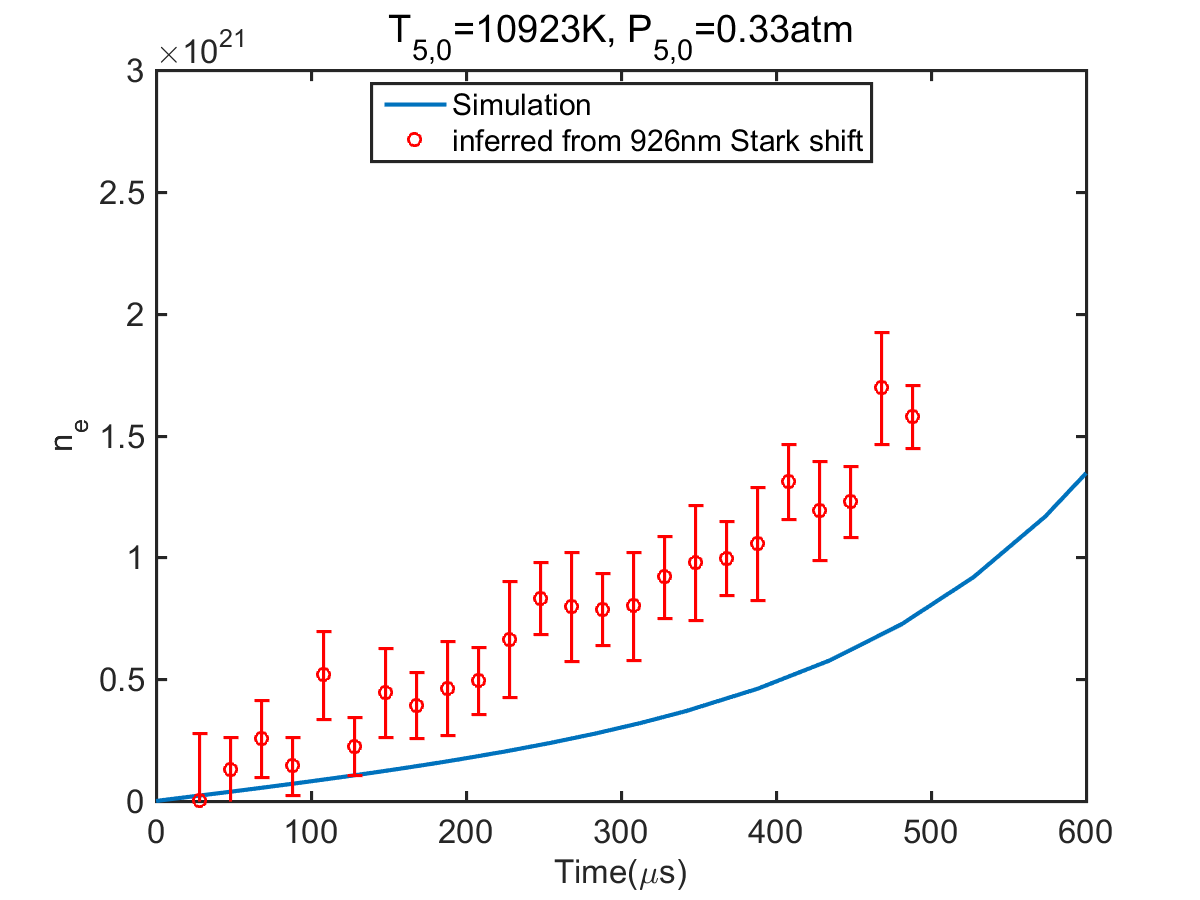
\includegraphics[width=\textwidth]{10923K_033atm_ne_sim_926.png}
      \caption{\label{fig:} }
      \end{subfigure}
        \begin{subfigure}[b]{0.4\textwidth}
     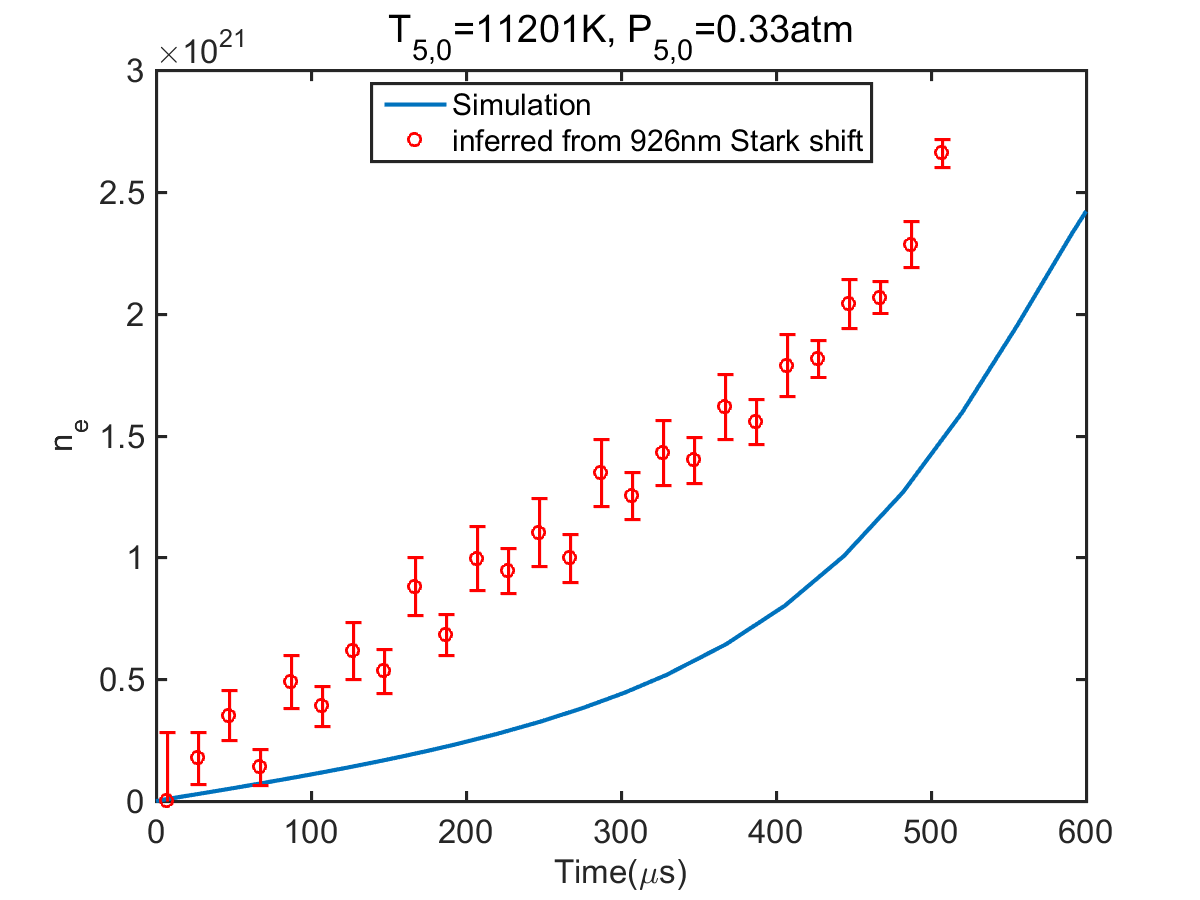
\includegraphics[width=\textwidth]{11201K_033atm_ne_sim_926.png}
      \caption{\label{fig:} }
      \end{subfigure}
    \caption{\label{fig:more_ne} The electron number density inferred from the 926 nm Stark shift (Symbols) and the simulations (Lines) from 10,150- 11,200 K.  Error bars represent the uncertainty of lineshape fit.}
\end{figure}

\section{Uncertainty Analysis}

The uncertainty of the current 926 nm Stark shift $n_e$ diagnostic method mainly includes the lineshape fitting uncertainty, the uncertainty of systematic experimental effects, and the uncertainty in the functional form of equation \ref{eq:stark_shift} and the Stark parameters in Table \ref{tab:Stark_parameters}.

The error bars in all the figures of the current paper represent the uncertainty from the Voigt lineshape fitting. The line-center fitting uncertainty is obtained from the Matlab ``lsqcurvefit" function with 95\% confidence interval. It is multiplied by $\sqrt{2}$ to represent the 95\% confidence interval of the relative Stark shift. This uncertainty is then propagated to the electron number density using the numerically calculated gradient of equation \ref{eq:stark_shift}, giving approximately 10 - 20\% electron number density uncertainty, as shown in figure \ref{fig:more_ne}.
   
As mentioned before, the uncertainty due to other line-center shift mechanisms is suppressed in the current experiment. The line-center of the first scan with a reliable Voigt fit behind the reflected shock wave is used as the reference for subsequent Stark shift measurements. Because the absolute van der Waals shift is incorporated in this line-center reference, only a relative change in the van der Waals shift could interfere with the Stark shift determination. The magnitude of this relative change of the van der Waals shift, and the corresponding error in the Stark shift,is estimated as follows.  The van der Waals FWHM for the 777 nm transition is approximately 0.015 cm$^{-1}$ according to the current study. The van der Waals shift may be estimated\cite{Konjevic2012} to be approximately 1/3 of FWHM value, giving 0.005 cm$^{-1}$. This value should vary linearly with small changes in pressure. During the test time the pressure change typically varies less than 5\%, resulting in a corresponding change in the van der Waals shift of less than 0.001 cm$^{-1}$, well below the Stark shift of 0.06 cm$^{-1}$. The Doppler shift is also small and neglected because the gases behind the reflected shock are usually assumed to be stagnated.

The major uncertainty sources of the current Stark shift measurements come from the systematic experimental effects such as the bias caused by the scan direction. This uncertainty is mitigated by careful optical alignment, choice of detector gain and data analysis. However, these effects are not completely eliminated and contribute approximately 10-20\% to the uncertainty in current electron number density determination.  

The most significant uncertainty source for the current diagnostic method originates from  the uncertainty of the Stark parameters in Table \ref{tab:Stark_parameters} and the functional form of equation \ref{eq:stark_shift}. These uncertainties are hard to quantify, especially at lower electron number density, due to the scarcity in both theoretical and experimental studies. Previous emission diagnostics suggest that there could be a 50\% discrepancy between the measured and the predicted Stark shift for some atomic oxygen transitions\cite{Baer1993_semiconductor, Goly1987}. 

Uncertainties for the experimental conditions are summarized below. The maximum shock velocity error for the current study is 0.5\%, which corresponds to a temperature uncertainty of about 1\%.  The pressure rise within the test time is minimized by a driver insert to be below 5\% within the test time for most cases. The rise time of the Kistler pressure transducer is on the order of  5 $\mu$s. Uncertainty in  determining time zero of is estimated to be $5\sqrt{2}\approx 7 \mu$s.


\section{Conclusion and Discussions}
In this work, we report a laser absorption measurement method and results for electron number density time-history, $n_e(t)$, based on the Stark shift of the O(3p $^5$P$_{3}$) to O(3d $^5$D$_{2,3,4}^0$) transition at 926 nm. This transition has a Stark width-to-shift ratio on the order of 1 and therefore its Stark shift is quite sensitive to the electron number density. 

The electron number density increased from 0 to $2\times10^{21}$m$^{-3}$ within 500 $\mu$s test time at T=11,200 K. A time-resolution of 20 $\mu s$ was readily achieved, with improvements possible by increasing the laser scanning rate. $n_e(t)$ inferred from the 926 nm Stark shift agrees with those inferred from the 777 nm Stark shift and Stark broadening, but is more sensitive to $n_e$ and robust to noise.

The measured $n_e(t)$ agreed with a previously developed collisional-radiative model\cite{Li2019_modeling} within a factor of 2 in general. Notably, the heavy particle and electron impact ionization rates of Ar in that model were $\sim$18 times larger than their nominal values found in the literature. The measured $n_e(t)$ could be used to improve details of this modeling in the future.

The $n_e$ diagnostic in the current paper has some limitations: 1.The Stark shift parameters in Table \ref{tab:Stark_parameters} and the function form of equation \ref{eq:stark_shift} need to be further studied theoretically and even better, calibrated by other well-established diagnostic method in the future. 2. Notably, a moderate amount of O(3p $^5$P$_{3}$), larger than 10$^{15}$/m$^3$, needs to exist in the system to achieve a reasonable SNR of the absorbance. For the current shock-heated 1\% O$_2$/Ar mixture, this limits the initial translational temperature range to be greater than 10,000K. This limit could be extended to lower temperature if the  O(3p $^5$P$_{3}$) population is in equilibrium or using cavity-enhanced absorption spectroscopy.

The current sensitive and robust electron number density diagnostic should prove useful for plasma studies involving oxygen atoms, especially when atomic hydrogen is not a naturally occurring element of the system, such as in aerothermodynamics modeling of high-enthaply air and plasma processing.  


\section*{Acknowledgement}
% \begin{acknowledgement}
The authors thank Prof. Mark A. Cappelli,  Dr. David F. Davidson, Prof. Leo Hollberg, Dr. Yu Wang and Dr. Jay B. Jeffries for helpful discussions.  This work was supported by the Air Force Office of Scientific Research (AFOSR) under grant number FA9550-16-1-0291, with Dr. Ivett Leyva as the technical monitor. 

\bibliographystyle{unsrt}
\bibliography{ne_diagnostics.bib}
% \end{acknowledgement}

\end{document}

